\graphicspath{{./03-Biblio/images/}}

\chapter{Analyses multi-échelles des milieux granulaires}
\label{chap:biblio}

%\epigraph{Si chacun de nous ajoute quelque chose au domaine commun, dans l'ordre de la science, de l'art ou de la moralité, c'est parce qu'une longue série de générations ont vécu, travaillé, pensé et souffert avant nous.}{Marcellin \textsc{Berthelot}, chimiste français (1827 - 1907)}

L'objectif du présent chapitre est de présenter certaines des connaissances déjà acquises et de décrire quelques travaux réalisés par la communauté scientifique dans les domaines de la mécanique des milieux granulaires, du traitement d'images issues de techniques d'imagerie 3D et de la simulation numérique de compression de poudres.
\\Dans un premier temps une analyse des phénomènes physiques propres aux matériaux granulaires sera faite et une description des poudres utilisées dans les expérimentations sera donnée. Ensuite, une présentation de la tomographie à rayons X, technique d'imagerie 3D, sera faite avant de décrire plus en détails les principes des travaux réalisés sur les images 3D. Enfin, les principales méthodes de simulation numérique concernant les matériaux granulaires seront présentées afin de mieux connaître les tenants et les aboutissants de chacune d'entre elles.

\section{Milieux granulaires}
	Les paragraphes qui suivent servent aux lecteurs non avisés concernant les milieux granulaires. Il s'agit de décrire certains phénomènes physiques en liaison avec ces milieux de manière à mieux les comprendre. Ce qui suit est basé sur les lectures de \citet{mollon_mecanique_2015}, \citet[Chapitres 1, 4 et 5]{matuttis_understanding_2014} et \citet{cambou_micromechanics_2009}.
	\subsection{Matériaux granulaires}
		\subsubsection{Quelques chiffres}
			Bien qu'on n'y fasse pas vraiment attention, les matériaux granulaires sont très présents dans nos vies. Chaque année dans le monde, l'industrie manipule plusieurs milliards de tonnes de matériaux granulaires. Un matériau granulaire intervient dans le cycle de fabrication d'un produit fini sur deux et la matière en grain représente, en masse, \si{70}{\%} des matières premières de l'industrie mondiale \citep{thomas_poudres_2012}. Par ailleurs, l'Union Nationale des Producteurs de Granulats estime qu'en $2016$ la production de granulats (matériaux pour la construction) en France était de \num{5.1} tonnes par habitant \citep{unpg}. On voit ici l'importance économique que porte ces matériaux et pourtant, il est encore aujourd'hui difficile de comprendre le comportement de ceux-ci. Il s'agit donc d'un important levier économique.
			\\Les matériaux granulaires ont également une grande importance en ce qui concerne les enjeux humains puisqu'environ \num{32000} victimes par an dans le monde sont à déplorer à cause de glissements de terrain \citep{petley_global_2012}. On comprend alors l'intérêt suscité dans le domaine du génie civil à la compréhension de ces matériaux.
		\subsubsection{Applications industrielles et thématiques de recherche}
			Comme mentionné dans le précédent paragraphe, les matériaux granulaires sont utilisés par de très nombreuses industries. Les principaux secteurs sont mentionnés ci-dessous.
			\begin{itemize}
				\item Industrie minière : extraction de matières premières dans les carrières et les mines.
				\item Génie civil : fabrication du ciment, interactions entre constructions et sols, terrassement.
				\item Industrie agroalimentaire : production de matière en grains (céréales, aliments en poudres, fruits, ...).
				\item Industrie pharmaceutique : broyage, mélange et compaction de produits actifs et excipients.
				\item Industrie chimique : réactions solides-solides et solides-liquides (grande surface d'échange liée à la surface spécifique des grains)
				\item industrie mécanique : compression de poudre, traitement et convoyage de petites pièces en grande quantité.
			\end{itemize}
			Au delà des industries, de nombreuses recherches sont menées afin de répondre à certaines problématiques environnementales et humaines liées aux matériaux granulaires. En voici quelques exemples :
			\begin{itemize}
				\item Catastrophes humaines et matérielles par instabilités de pentes, activités volcaniques et sismiques. Les instabilités de terrains (glissements de terrains, avalanches) sont des écoulements granulaires et des efforts sont faits pour comprendre leurs déclenchement, propagation et arrêt. Les coulées volcaniques, sont des écoulements aérosols avec des températures et vitesses élevées. Encore une fois, la dynamique de ces coulées fait l'objet de nombreuses recherches. Enfin, un gros effort est également fourni afin de comprendre la propagation des ondes dans les matériaux granulaire pour mieux comprendre les phénomènes sismiques. Quoi qu'il en soit, de gros moyens sont mis en place afin de mettre en \oe{}uvre et dimensionner des systèmes de protection.
				\item \'Etude de la dynamique fluviale, littorale et des dunes de sable par sédimentologie. Les interactions entre fluide et milieu granulaire sont étudiés afin de comprendre l'équilibre dynamique dans le domaine de l'hydrologie. De même pour les interactions, complexes, entre topographie et climat pour comprendre la formation et le déplacement des dunes de sable.
				\item Compréhension de phénomènes physiques. La compréhension de phénomènes propres aux milieux granulaires (ségrégation, formation de motifs périodiques, corrugation, ...) est à l'origine de nombreuses études souvent simplifiées à l'extrême (grains sphériques de même taille). Enfin, les planétologues font souvent appel à l'étude de la matière en grains afin de mieux comprendre les cratères d'impacts, les anneaux de Saturne ou encore optimiser le déplacement des rovers sur les sols des planètes explorées.
			\end{itemize}
	\subsection{Mécanique des milieux granulaires confinés}
		\subsubsection{Propriétés et spécificités}
			En sciences des matériaux, on entend parler de trois états de la matière : l'état solide, l'état liquide et l'état gazeux. Le but ici n'est pas de décrire chacun de ces états de la matière mais de comprendre où placer les milieux granulaires qui sont constitués de particules solides mais qui s'écoulent à la manière des liquides. La matière en grains a en effet des propriétés très différentes de la matière dite continue. Ces spécificités, d'ordre géométrique, mécanique et physico-chimique, sont à l'origine des difficultés de modélisation rencontrées lorsqu'on s'intéresse aux matériaux granulaires.
			\\La première spécificité des milieux granulaires est qu'il n'existe pas d'équation universelle comme pour les matériaux plus "classiques". En effet, l'élasticité donne la loi de Hooke pour les matériaux solides déformables. Il en va de même avec l'équation de Navier-Stokes pour les fluides newtoniens. Quand ces matériaux continus ne sont pas élastiques et que les fluides sont non-newtoniens, il est possible de faire évoluer ces lois en ajoutant des paramètres par exemple. En ce qui concerne les matériaux granulaires, il n'existe pas encore de loi universelle du comportement de la matière. On se base donc généralement sur des fondements empiriques et sur des théories plus ou moins abouties souvent contraignantes (géométrie des grains, régime d'écoulement, loi de contact, type de matériau).
			\\Le grand nombre de particules dans un tel milieu le rend également spécifique. Le fait d'être en présence d'un très grand nombre de solides de très petites tailles engendre une surface de contact accessible totale, appelée surface spécifique, très grande. Du fait de cette caractéristique, de très nombreux contacts physiques et interactions physico-chimiques s'établissent entre les particules. Cela rend le milieu granulaire plus complexe à étudier. Par exemple, les approches macroscopiques basées sur la conservation d'énergie ne sont plus valables puisque le milieu dissipe énormément d'énergie à l'échelle des grains.
			\\Enfin, il existe une autre spécificité du milieu granulaire : il est difficile de séparer l'échelle du grain de l'échelle globale du système de grains. En ce qui concerne les matériaux continus plus classiques, les chercheurs et ingénieurs s'intéressent très souvent à des comportements significatifs qui se situent à une échelle très largement supérieure à celle des particules élémentaires. Dans les milieux granulaires, il est très difficile d'étudier un ensemble de particules de manière exacte en ignorant soit l'échelle des particules, soit l'échelle globale du système. En voici un exemple : une bande de cisaillement d'épaisseur équivalente à quelques grains peut engendrer le glissement de plusieurs millions/milliards de grains se situant d'un côté ou de l'autre de la bande de glissement. Le phénomène est ici à la fois local (bande de cisaillement étroite) et global (déplacement d'une grande masse de particules).
		\subsubsection{Phénoménologie}
			On peut, de manière générale, considérer deux grandes familles de matériaux granulaires qui dépendent de la taille et de la nature des particules constituant le milieu :
			\\\vspace{1mm}\\
			\begin{minipage}[c]{0.24\linewidth}
				\includegraphics[width=\textwidth]{poudre_fine_shipton-mill.jpg}
			\end{minipage}\hfill
			\begin{minipage}[c]{0.74\linewidth}
				\begin{itemize}
					\item \emph{Les milieux granulaires "fins" ou poudres} dont les particules sont de tailles inférieures ou approximant le micromètre. Des forces cohésives existent généralement entre les particules (Van Der Waals, électrostatiques, capillaires) et les interactions avec le fluide environnant (eau, air, ...) sont à prendre en compte. L'étude des poudres nécessite de prendre en compte la physico-chimie en plus de l'approche purement mécanique. (Source photo : \url{www.shipton-mill.com}).
				\end{itemize}
			\end{minipage}\vspace{5mm}
			\begin{minipage}[c]{0.24\linewidth}
				\includegraphics[width=\textwidth]{graviers_unpg.jpg}
			\end{minipage}\hfill
			\begin{minipage}[c]{0.74\linewidth}
				\begin{itemize}	
					\item \emph{Les milieux granulaires "grossiers"} dont les particules ont des tailles généralement supérieures à la centaine de micromètres. Les grains vont alors être soumis à la gravité et aux forces de contacts des particules voisines (appuis, frottements, chocs). Une approche purement mécanique suffit à étudier le milieu. Malgré cette avantage par rapport aux poudres fines, il reste difficile de bien comprendre ces milieux pulvérulents. (Source photo : \url{www.unpg.fr})
				\end{itemize}
			\end{minipage}\vspace{5mm}
			En fonction de la famille d'appartenance du milieu granulaire, certains phénomènes sont à prendre en compte et d'autres non. Les paragraphes qui suivent donnent une liste de ces phénomènes. Comme ces derniers dépendent de nombreux paramètres, il ne sera pas spécifié les conditions d'obtention de manière précise mais plutôt de manière générale.
			\subparagraph{Interactions en surface -}
				Pour les particules les plus grossières, l'interaction entre surfaces de grains est principalement due à la déformation élastique pour la composante normale et à la friction de Coulomb pour la composante tangentielle. Lorsque les particules sont plus fines, d'autres interactions peuvent intervenir. Dans un environnement fortement humide, les petits grains vont interagir entre eux par l'intermédiaire d'une force de cohésion liée à l'agglomération de molécules d'eau au niveau des contacts. Dans un environnement sec en revanche, des effets électrostatiques peuvent apparaître s'il existe un mouvement relatif entre les grains. Tous ces effets de surface vont avoir une importance cruciale sur le comportement du milieu granulaire. Il est à noter que ces interactions sont dépendantes de la taille des grains\footnote{Cela ne concerne pas les forces "mécaniques" mais plutôt les forces d'adhésion (capillaires, Van der Waals, ...).}, de leur nature et de l'environnement. Si la nature des grains reste invariante, l'environnement et la taille des grains, eux, peuvent varier au cours du temps (climat, fractures des grains, frittage, ...).
			\subparagraph{Friction et dissipation d'énergie -}\label{para03:friction}
				Les effets de friction et de dissipation contribuent aux interactions entre grains mais mènent également à des comportements macroscopiques qui diffèrent de celui des systèmes d'atomes et de molécules. Dans un milieu dense, les frottements aux interfaces du milieu granulaire joue un rôle important et expliquent par exemple les effets d'arche qui seront présentés dans un prochain paragraphe.
			\subparagraph{Géométrie des particules, roulement et glissement -}\label{para03:glissement}
				En fonction de la géométrie des grains, le comportement du milieu granulaire peut drastiquement changer. Ici le terme géométrie décrit uniquement la forme des grains et non leur taille. Le fait que les particules aient des formes complexes ou non va également jouer sur le comportement du milieu. Un milieu constitué uniquement de grains sphériques facilitera l'analyse (puisqu'on peut considérer les symétries et diminuer le nombre de variables pour la modélisation) mais sera moins approprié pour l'étude de certains phénomènes physiques. En effet, pour des particules sphériques les surfaces de contact sont minimisées et les effets liés à la friction et à la cohésion seront également minimisés puisque les efforts de contact seront normaux aux surfaces. Ainsi, un tel milieu mettra l'accent sur le roulement aux dépends du glissement si aucun coefficient de frottement n'est considéré. Lors d'un réarrangement de grains, la dissipation d'énergie est minimale. \`A l'inverse, un milieu pour lequel les particules ont des formes complexes présentera des surfaces de contacts également plus complexes et il existe naturellement un équilibre entre glissement et roulement. De tels milieux vont permettre d'observer ce qui a été décrit dans le paragraphe précédent sur la friction et la dissipation d'énergie. Cet effet est observable sur la figure \ref{fig03:shape_effect}.
				\begin{figure}\centering
					\begin{minipage}[c]{0.47\textwidth}
						\subfloat[]{
							\includegraphics[width=\textwidth]{heap_hex.png}
							\label{subfig03:shape_effect_hex}
						}
					\end{minipage}\hspace{0.04\textwidth}
					\begin{minipage}[c]{0.47\textwidth}
						\subfloat[]{
							\includegraphics[width=\textwidth]{heap_circ_init.png}
							\label{subfig03:shape_effect_circ_init}
						}\\
						\subfloat[]{
							\includegraphics[width=\textwidth]{heap_circ_final.png}
							\label{subfig03:shape_effect_circ_final}
						}
					\end{minipage}
					\caption{\label{fig03:shape_effect}Effet de la forme des particules sur la formation d'un tas : (a) les particules polyédriques se stabilisent grâce à l'effet de la friction lors du glissement ;  (b) lorsqu'un empilement de particules sphériques et créé, (c) ces dernières roulent sans glisser et se dispersent dans l'espace \citep{matuttis_understanding_2014}.}
				\end{figure}
			\subparagraph{Effet d'arche -}
				L'effet d'arche se caractérise lorsque des forces normales à la direction de chargement apparaissent. Dans les milieux granulaires, ce phénomène est très présent et est utilisé depuis des milliers d'années dans la construction. Lorsque le milieu granulaire est confiné entre des parois, les grains vont engendrer des forces liées au frottement grain/grain et grain/paroi. Ces forces vont être propagées de grain en grain formant ce qu'on appelle une chaîne de forces. Le chemin suivi par les chaînes de forces dépend des contacts qui existent entre les grains (nombre, surface et direction des contacts). En général, les chaînes de forces dévient rapidement de la direction de sollicitation produisant ainsi des forces radiales. Cet effet explique l'importance des efforts de frottements entre un ensemble de grains soumis à son propre poids et les parois d'un silo à grain.
			\subparagraph{Dilatance de Reynolds -}\label{para03:dilatance}
				Le phénomène de dilatance est observable dans un milieu granulaire en compression dans lequel des contraintes de cisaillement sont présentes. Il est possible d'illustrer le phénomène par un essai de compression triaxiale (\textit{c.f.} paragraphe \ref{para03:triax}) bien que la dilatance se manifeste dans d'autres cas. Lors d'un confinement isotrope, les grains se réarrangent et se déforment de la même manière quelque soit la direction (en moyenne en tout cas) : il y a une densification du milieu (volume qui diminue et résistance mécanique qui augmente). Si maintenant la compression augmente suivant une direction mais reste constante suivant les autres (pression de confinement constante avec chargement axial), alors les grains, qui se déplacent majoritairement dans l'axe de compression, sont confrontés à deux types de résistances : les forces de frottements intergranulaires et la résistance liée au manque d'espace avec les grains voisins. Lorsque l'effort de cisaillement est suffisamment grand pour contrecarrer ces résistances au mouvement, un réarrangement des grains se fait remarquer. C'est ce réarrangement, moins ordonné, des grains qui génère une augmentation du volume qui correspond au phénomène de dilatance. La figure \ref{fig03:dilatance} aide à comprendre le réarrangement des grains lorsque des efforts de cisaillement interviennent. La dilatance dans un milieu granulaire est également une des causes de l'effet d'arche.
				\begin{figure}\centering
					\begin{minipage}[c]{0.4\textwidth}\centering
						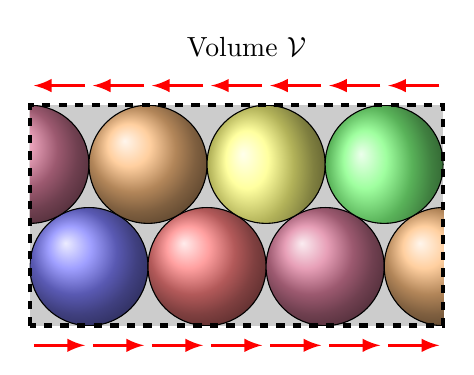
\begin{tikzpicture}[scale=.5]
							% Dessine le volume
							\fill[gray!40] (-1.5,-1.5) rectangle ++(10.5,{3+3*sin(60)});
							\begin{scope}
								\clip (-1.5,-1.5) rectangle ++(10.5,{3+3*sin(60)});
								% Dessine les grains du bas
								\filldraw[ball color=blue!50] (0,0) circle (1.5);
								\filldraw[ball color=red!50] (3,0) circle (1.5);
								\filldraw[ball color=purple!50] (6,0) circle (1.5);
								\filldraw[ball color=orange!50] (9,0) circle (1.5);
								% Dessine les grains du haut
								\filldraw[ball color=purple!50] (120:3) circle (1.5);
								\filldraw[ball color=orange!50] (60:3) circle (1.5);
								\filldraw[ball color=yellow!50] (3,0) ++(60:3) circle (1.5);
								\filldraw[ball color=green!50] (6,0) ++(60:3) circle (1.5);
							\end{scope}
							% Dessine le cadre du volume et écrit
							\draw [ultra thick, dashed] (-1.5,-1.5) rectangle ++(10.5,{3+3*sin(60)});
							\path (4,{2.5+3*sin(60)}) node [above]{Volume $\mathcal{V}$};
							% Dessine le chargement
							\foreach \x in {8.9,7.4,...,-0.1} {
								\draw[very thick, -latex, red] (\x,{2+3*sin(60)}) -- ++(-1.3,0);}
							\foreach \x in {-1.4,0.1,...,7.6} {
								\draw[very thick, -latex, red] (\x,-2) -- ++(1.3,0);}
						\end{tikzpicture}
					\end{minipage}
					\begin{minipage}[c]{0.18\textwidth}\centering
						~\\\vspace{5mm}~\\
						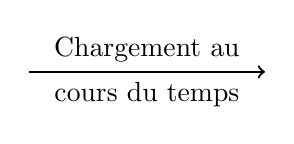
\begin{tikzpicture}
							\draw[thick, ->] (0,0) -- (3,0) node[midway, above] {Chargement au} node[midway, below]{cours du temps};
						\end{tikzpicture}
					\end{minipage}
					\begin{minipage}[c]{0.4\textwidth}\centering
						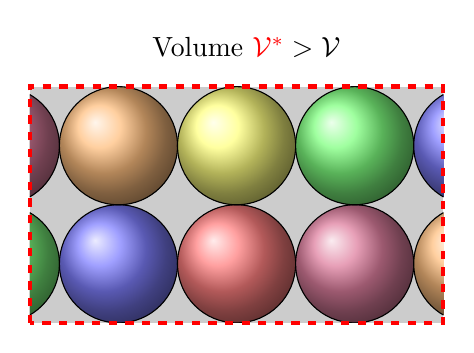
\begin{tikzpicture}[scale=.5]
							% Dessine le volume
							\fill[gray!40] (-1.5,-1.5) rectangle ++(10.5,6);
							\begin{scope}
								\clip (-1.5,-1.5) rectangle ++(10.5,6);
								% Dessine les grains du bas
								\filldraw[ball color=green!50] (-3+.75,0) circle (1.5);
								\filldraw[ball color=blue!50] (0.75,0) circle (1.5);
								\filldraw[ball color=red!50] (3.75,0) circle (1.5);
								\filldraw[ball color=purple!50] (6.75,0) circle (1.5);
								\filldraw[ball color=orange!50] (9.75,0) circle (1.5);
								% Dessine les grains du haut
								\filldraw[ball color=purple!50] (-3+.75,3) circle (1.5);
								\filldraw[ball color=orange!50] (.75,3) circle (1.5);
								\filldraw[ball color=yellow!50] (3.75,3) circle (1.5);
								\filldraw[ball color=green!50] (6.75,3) circle (1.5);
								\filldraw[ball color=blue!50] (9.75,3) circle (1.5);
							\end{scope}
							% Dessine le cadre du volume et écrit
							\draw [ultra thick, dashed, red] (-1.5,-1.5) rectangle ++(10.5,6);
							\path (4,5) node [above]{Volume ${\color{red}\mathcal{V^*}} > \mathcal{V}$};
						\end{tikzpicture}
					\end{minipage}
					\caption{\label{fig03:dilatance}Illustration du phénomène de dilatance : l'état initial (à gauche) est plus dense que l'état après chargement (à droite). Cela ne se produit que pour des efforts de cisaillement assez importants au sein du milieu granulaire.}
				\end{figure}
			\subparagraph{Formation de bandes de cisaillement -}\label{para03:bande_cisaillement}
				Lorsqu'un milieu granulaire est comprimé de manière non isotrope, des contraintes de cisaillement font leur apparition dans certaines zones. Comme il l'a été dit dans le paragraphe précédent, l'apparition de contraintes de cisaillement dans un milieu confiné engendre également un effet de dilatance. Ainsi, dans les zones où les contraintes de cisaillement atteignent une valeur relativement grande, les grains vont avoir tendance à se désenchevêtrer et diminuer la densité du milieu localement. Généralement cela se passe sur un plan ayant une épaisseur de quelques grains qu'on appelle bande de cisaillement. Lorsque la densité diminue, la résistance mécanique diminue également et les zones de cisaillement deviennent finalement les zones de rupture, on entend souvent parler de bande de glissement puisqu'une partie située d'un côté de la bande va glisser sur la partie située de l'autre côté. La figure \ref{fig03:cisaillement} montre l'apparition d'une bande de cisaillement observée par tomographie à rayons X (cf. paragraphe \ref{para03:tomo}) lors d'un essai de compression triaxiale (cf. paragraphe \ref{para03:triax}). La figure \ref{subfig03:cisaillement_02} est issue de la corrélation d'images 3D (cf. paragraphe \ref{para03:DIC}) et montre les déformations déviatoires permettant ainsi de distinguer clairement la bande de cisaillement.
			\begin{figure}\centering
				\subfloat[]{
					\includegraphics[height=0.3\linewidth]{bande_cisaillement_00.jpg}
					\label{subfig03:cisaillement_00}}\hspace{1.5cm}
				\subfloat[]{
					\includegraphics[height=0.3\linewidth]{bande_cisaillement_01.jpg}
					\label{subfig03:cisaillement_01}}\hspace{1.5cm}
				\subfloat[]{
					\includegraphics[height=0.26\linewidth]{bande_cisaillement_02.jpg}
					\label{subfig03:cisaillement_02}}
				\caption{\label{fig03:cisaillement}Reconstructions de tomographie montrant la formation d'une bande de cisaillement dans un ensemble de grains (a) à l'état initial avant chargement et (b) à l'état final après chargement. (c) On distingue encore mieux la bande grâce à la corrélation d'images (illustrations issues des travaux de  \cite{kawamoto_all_2018}).}
			\end{figure}
	\subsection{Essais de compression dédiés aux milieux granulaires}
		De manière générale, les matériaux granulaires ne forment plus un système solide à partir d'une certaine contrainte en traction qui élimine tout effort de cohésion intergranulaire. C'est la raison pour laquelle l'étude de ces milieux en équilibre statique s'intéresse en grande partie aux états confinés. On retrouvera certains éléments qui suivent dans les lectures de \citet{terzaghi_soil_1996} et \citet{bardet_experimental_1997}.
		\subsubsection{Les essais de compression}
			Nous allons voir dans les paragraphes qui suivent, deux méthodes couramment utilisées pour étudier le comportement mécanique des poudres dans des espaces confinés. Ces essais sont bien connus des géotechniciens qui caractérisent les sols régulièrement avec ces techniques. Nous considérerons que l'échantillon est axisymétrique (d'où les termes "de révolution") et que la direction axiale est la direction de l'axe de symétrie tandis que les directions radiales sont les directions normales à cet axe. Lorsqu'on s'intéresse à la mécanique des milieux granulaires, il est plus facile d'utiliser la convention utilisée en géotechnique qui consiste à considérer les contraintes de compression positives alors que la traction est négative.
			\paragraph{Compression \oe{}dométrique de révolution\\}
				L'essai de compression \oe{}dométrique est également appelé essai de consolidation ou de compressibilité. Il permet d'apprécier la déformation axiale d'un échantillon dont les parois latérales sont fixes et rigides de manière à ne pas se déformer sous l'action des efforts traversant l'échantillon. Un schéma de principe est donné sur la figure \ref{fig03:oedometre}. Avec cet essai, la déformation de l'échantillon est uniquement axiale et il est possible de mesurer la force appliquée dans la direction axiale, le déplacement appliqué dans la même direction mais aussi dans certains cas la pression exercée par l'échantillon sur les parois latérales. Ainsi, en reprenant les notations fournies à la page \pageref{keywords}, après mise en chargement on a :
				\begin{equation}\label{eq03:defo_oedometre}
					\left\{\begin{array}{l}
						\varepsilon_a (= \varepsilon_{33}) \neq 0\\
						\varepsilon_r (= \varepsilon_{11} = \varepsilon_{22}) = 0\\
						\gamma_{12} = \gamma_{13} = \gamma_{23} = 0
					\end{array}\right.
				\end{equation}
				\begin{figure}\centering
					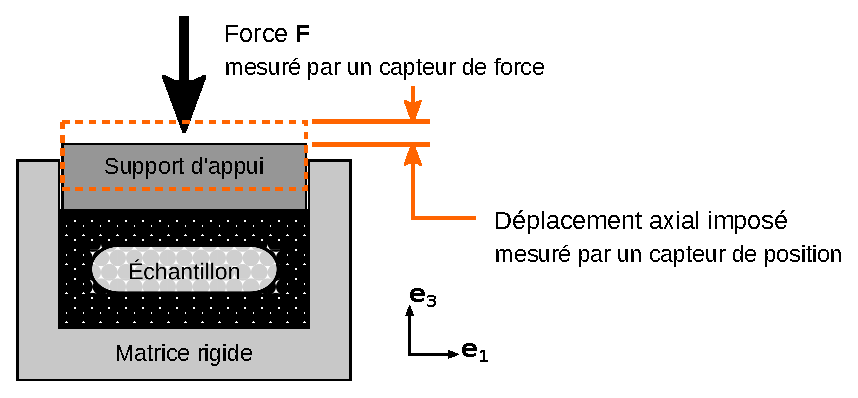
\includegraphics[scale=0.9]{oedometre.eps}
					\caption{\label{fig03:oedometre}Principe du test de consolidation}
				\end{figure}
				Cet essai peut également être réalisé avec drainage. La circulation d'un fluide est alors permise et ce dernier est drainé vers l'extérieur du moule. Cela permet d'observer l'effet du tassement sur un milieu plus ou moins saturé (exemple : un sol saturé en eau).
			\paragraph{Compression triaxiale de révolution\\}\label{para03:triax}
				De manière générale un matériau granulaire est dans un état confiné. Cela veut dire que la contrainte moyenne dans le milieu constitue un état de compression, donc positive. Par décomposition du tenseur des contraintes (\ref{eq03:contraintes_triax}), on peut dire qu'il existe une contrainte de compression hydrostatique (donc isotrope), qui est la contrainte moyenne $p$, positive mais également des contraintes déviatoires qui modifient la géométrie du milieu. L'ensemble des contraintes déviatoires forme le déviateur des contraintes $\doubleunderline{\sigma_d}$. La contrainte déviatoire $q$ est couramment utilisée afin de déterminer la contribution des efforts qui ne modifient pas le volume du système. Par définition, cette contrainte déviatoire $q$ correspond à la contrainte équivalente de Von Mises calculée à partir du tenseur des contraintes déviatoires. Pour un système en contraintes axisymétriques (ce qui est le cas pour l'essai de compression triaxiale), $q$ correspond à la différence, en valeur absolue, de la contrainte axiale $\sigma_a$ et de la contrainte radiale $\sigma_r$. Si l'axe $3$ correspond à la direction axiale, alors:
				\begin{equation}\label{eq03:contraintes_triax}
					\begin{array}{l}
						\doubleunderline{\sigma} = p\cdot\doubleunderline{I} + \doubleunderline{\sigma_d}\\
						\\
						q = \sqrt{\cfrac{3}{2}\;\mathrm{tr}(\doubleunderline{\sigma_d}^2)}
					\end{array}
					\quad\text{avec}\quad\begin{array}{rcl}
					p & = & \text{tr}(\doubleunderline{\sigma})/3\vspace{0.3cm} = (\sigma_{11}+\sigma_{22}+\sigma_{33})/3\\
					\doubleunderline{\sigma_d} & = &
					\begin{pmatrix}
						\sigma_{11}-p & \sigma_{12} & \sigma_{13} \\
						\sigma_{12} & \sigma_{22}-p & \sigma_{23} \\
						\sigma_{13} & \sigma_{23} & \sigma_{33}-p \\
					\end{pmatrix}\end{array}
				\end{equation}
				\indent L'essai de compression triaxiale consiste à déterminer les états de contraintes et déformations de l'échantillon lorsque ce dernier est chargé de manière axiale et radiale. Le chargement axial se fait de la même manière que pour l'essai de compression \oe{}dométrique, un piston vient exercer une force à l'extrémité de l'échantillon. On peut choisir de piloter soit la force appliquée par le piston, soit la vitesse de déplacement du piston. Le chargement radial est quant à lui exercé par l'intermédiaire d'un fluide mis sous pression. En fait, le dispositif ne permet pas de créer un chargement uniquement radial en plus du chargement axial, il crée un chargement isotrope. Pour cela, une membrane souple est placée aux extrémités de l'échantillon de manière à l'isoler du fluide environnant, il faut donc une membrane étanche et suffisamment souple pour ne pas rigidifier l'échantillon. Le fluide qui englobe complètement l'échantillon est mis sous pression de manière à exercer cette pression sur la membrane, et donc sur le matériau à tester. La contribution de ce chargement est uniquement isotrope puisqu'il s'agit d'une pression hydrostatique. Un schéma du principe de l'essai est donné dans la figure \ref{fig03:triax}. Les membranes sont très souvent des membranes en élastomère (latex, néoprène, ...). L'eau ou l'huile sont régulièrement utilisés comme fluides mis en pression.
				\begin{figure}\centering
					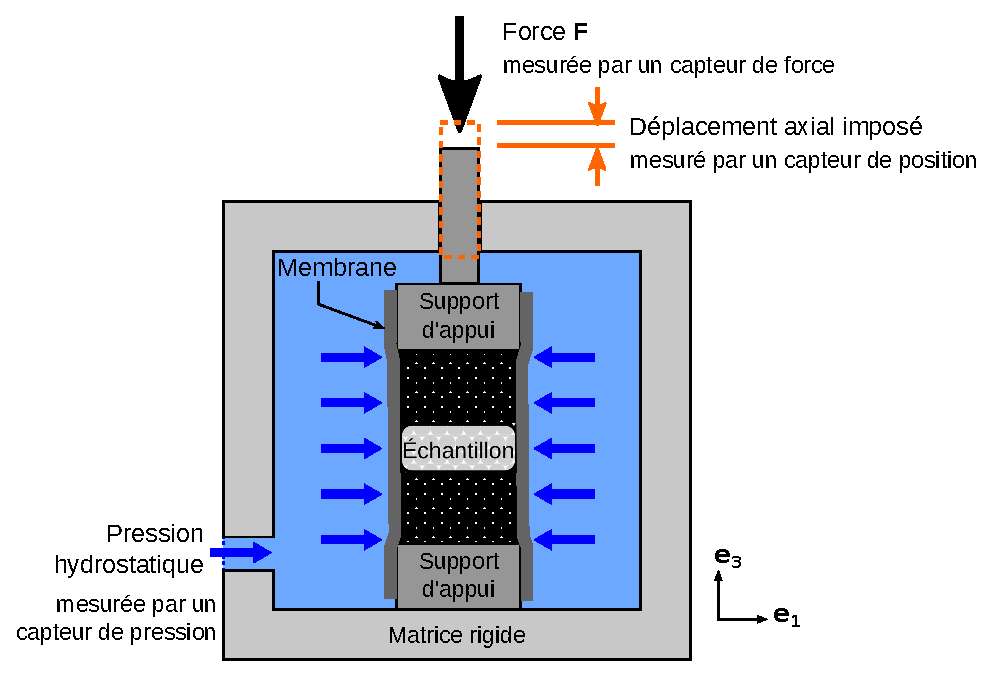
\includegraphics[scale=0.9]{triax.eps}
					\caption{\label{fig03:triax}Principe de l'essai de compression triaxiale}
				\end{figure}
				\\La compression triaxiale de révolution à l'avantage d'être plus riche en terme d'information que l'essai de consolidation. En effet, le chargement radial étant imposé et l'échantillon étant accessible dans une cellule, il est possible d'obtenir la cinématique de l'ensemble et de connaître les efforts que subit la surface extérieure de l'échantillon, que ce soit dans les directions radiales ou axiale. Un autre avantage de cet essai par rapport à l'essai \oe{}dométrique est la possibilité de s'affranchir du frottement contre la paroi avec l'utilisation d'une membrane souple qui se déforme avec le milieu testé. On voit ici que la pression appliquée par le fluide influence la contrainte moyenne $p$ dans l'échantillon. Le chargement axial va, lui, influencer à la fois la contrainte moyenne $p$ mais aussi et surtout la contrainte déviatoire $q$. Ainsi, il est simple avec ce test de créer plusieurs chemins de chargement afin d'observer les effets de la contrainte moyenne de compression et de la contrainte déviatoire.
				\\Contrairement à la compression \oe{}dométrique où l'on observe la relation (\ref{eq03:defo_oedometre}), dans le cas de l'essai triaxial, si l'axe $3$ correspond à la direction axiale, on a :
				\begin{equation}\label{eq03:defo_triax}
					\left\{\begin{array}{l}
						\varepsilon_a (=\varepsilon_{33}) \neq 0\\
						\varepsilon_r (=\varepsilon_{11} =\varepsilon_{22}) \neq 0\\
						\gamma_{13} = \gamma_{23} \neq 0\\
						\gamma_{12} = 0
					\end{array}\right.
				\end{equation}
				Il est possible de décomposer le tenseur des déformations de la même manière que pour le tenseur des contraintes. Ainsi, nous parlerons de la déformation volumique $\varepsilon_v$ qui définit la part des déformations qui modifient le volume de l'échantillon et du déviateur des déformations $\doubleunderline{\varepsilon_d}$ qui définit les déformations impliquant un changement de géométrie de l'échantillon. On aura tendance, plus particulièrement, à parler de la déformation déviatoire $\varepsilon_d$ qui est définie de la manière indiquée ci-dessous. Si la direction \num{3} correspond à la direction axiale alors :
				\begin{equation}\label{eq03:decomposition_defo_triax}
					\begin{array}{l}
						\doubleunderline{\varepsilon} = \cfrac{1}{3}\;\varepsilon_v\cdot\doubleunderline{I} + \doubleunderline{\varepsilon_d}\\\\
						\varepsilon_d = \sqrt{\cfrac{2}{3}\;\mathrm{tr}(\doubleunderline{\varepsilon_d}^2)}
					\end{array}
					\quad\text{avec}\quad\begin{array}{rcl}
					\varepsilon_v & = & \text{tr}(\doubleunderline{\varepsilon})\vspace{0.3cm} = \varepsilon_{11}+\varepsilon_{22}+\varepsilon_{33}\\
					\doubleunderline{\varepsilon_d} & = &
					\begin{pmatrix}
					\varepsilon_{11}-\varepsilon_v/3 & \gamma_{12} & \gamma_{13} \\
					\gamma_{12} & \varepsilon_{22}-\varepsilon_v/3 & \gamma_{23} \\
					\gamma_{13} & \gamma_{23} & \varepsilon_{33}-\varepsilon_v/3 \\
					\end{pmatrix}\end{array}
				\end{equation}
				Pour des petits incréments de déformation, la déformation volumique $\varepsilon_v$ donne une très bonne approximation du rapport $(\mathrm{d}V-\mathrm{d}V_0)/\mathrm{d}V$ avec $\mathrm{d}V_0$ et $\mathrm{d}V$, respectivement, les volumes élémentaires avant et après déformation.
				\\\indent Comme avec le test de consolidation, il est possible d'observer l'effet du drainage d'un fluide circulant dans l'échantillon. On parlera d'essai de compression triaxiale drainé lorsque c'est le cas, ou non drainé dans le cas contraire.
		\paragraph{Compression de particules ductiles\\}
			Le comportement mécanique des particules qui constituent un milieu granulaire joue un rôle important dans le comportement mécanique de l'ensemble du milieu. C'est en effet la réponse mécanique de chacun des grains qui va dicter la réponse de l'ensemble de grains.
			\\Lorsque des particules présentant une rigidité élevée sont introduites et comprimées dans un moule et qu'elles ne sont pas soumises à des efforts engendrant leur fracture, ce sont essentiellement les chaînes de forces qui se créent dans le milieu qui va dicter la réponse mécanique du milieu granulaire. Dans ce cas, la géométrie des grains et la friction entre les grains et les parois du moule sont des facteurs très influents concernant les propriétés mécaniques du milieu.
			\\Dans le cas où le milieu pulvérulent est constitué de grains ductiles, c'est à dire capables de se déformer assez largement à un certain niveau de contraintes, alors la déformation des grains joue un rôle crucial dans la réponse mécanique de l'ensemble de grains. En effet, l'énergie de déformation nécessaire à la déformation des particules prend part dans le bilan énergétique et certains phénomènes vont être plus ou moins marqués. Par exemple, \citet{pavier_caracterisation_1998} montre que la dilatance de Reynolds est difficile à observer dans le cas d'un matériau constitutif ductile. En l'absence d'une surconsolidation élevée, la déformation des grains sous cisaillement permet le glissement des grains entre eux sans avoir à s'écarter. Les déformations vont être les plus grandes au niveau des zones de contact puisqu'il s'agit des zones où les contraintes sont le plus présentes. Ces déformations, au niveau des zones de contacts, vont élargir les surfaces de contacts et les effets liés aux frottements des grains vont être moins présents puisque les glissements inter-grains sont alors plus limités.
		\paragraph{}
			Il a été précédemment montré l'importance de la nature des particules constituant le milieu granulaire sur son comportement mécanique. Il est donc essentiel de connaître les propriétés du matériau constitutif afin de comprendre le comportement d'un système de grains. La partie qui suit à pour objectif de présenter les propriétés du matériau utilisé dans les travaux présentés ici : le polystyrène.
	\subsection{Comportement des particules polymériques}
		Cette partie a pour objectif de présenter le matériau granulaire concerné dans cette thèse. Comme il l'a été expliqué au chapitre \ref{chap:intro}, l'étude portera uniquement sur le matériau modèle et non sur des grains d'amidon, qui historiquement constituait le matériau d'étude. Afin d'informer le lecteur sur le matériau amidon, l'annexe \ref{annexe:amidon} présente les principales propriétés de celui-ci. Les propriétés mécaniques de l'amidon peuvent être analysées afin de déterminer les similitudes et différences avec le matériau modèle présenté ci-dessous.
		\\Les particules étudiées dans les travaux qui suivent sont des grains de polystyrène (pouvant être abrégé "PS" par la suite). Le polystyrène a un comportement mécanique typique des polymères. Avant de commencer à présenter ce matériau, une courte explication du comportement des polymères est nécessaire.
		\subsubsection{Polymères}
		Un polymère est un matériau organique constitué d'un ensemble de macromolécules, elles-mêmes constituées d'un certain enchaînement d'éléments structurants, appelés monomères, composés de chaînes carbonées. Les matériaux polymères font partie d'une très grande famille de matériaux. Il existe différentes sous-familles de polymères : le classement trouvé le plus souvent dans les ouvrages différencie les thermoplastiques, les thermodurcissables et les élastomères. Il s'agit là d'un classement assez global qui tient compte de nombreuses propriétés thermomécaniques : les thermoplastiques, une fois chauffés, sont malléables et facilement mis en forme, les thermodurcissables durcissent de manière irréversible sous l'action de réactifs et/ou d'un environnement favorisant (chaleur, lumière, ...) et les élastomères sont capables de se déformer de manière réversible jusqu'à de grandes, voire très grandes, déformations. Il est également possible de différencier les polymères par d'autres moyens : nature chimique, "forme" de la macromolécule, formulation chimique, arrangement cristallographique, etc. De par leurs natures très variées, les polymères peuvent avoir des comportements mécaniques très différents. De manière générale, les propriétés mécaniques des polymères dépendent d'au moins deux facteurs :
		\begin{itemize}
			\item le temps : les relations entre contraintes $\sigma$ et déformations $\varepsilon$ sont dépendantes de la vitesse de chargement $\dot{\sigma}$ et de la vitesse de déformation $\dot{\varepsilon}$. Cette propriété introduit le caractère visqueux des polymères.
			\item la température : il existe des transitions de phases pour certaines températures. Par exemple, la température de transition vitreuse définit les intervalles de températures pour lesquelles le matériaux passe d'un état caoutchouteux à un état de solide rigide. Le caractère visqueux des polymères est très dépendant de la température.
		\end{itemize}
		On ne peut pas dire qu'un matériau polymère soit un matériau répondant uniquement à la loi de Hooke, à la théorie de la plasticité ou à la loi de la viscosité des fluides. Afin d'étudier ces matériaux, il est plutôt judicieux de s'intéresser à la viscoélasticité et la viscoplasticité pour mieux comprendre l'écoulement des polymères : on entre dans le domaine d'étude de la rhéologie. Plusieurs modèles rhéologiques existent pour décrire au mieux le comportement des polymères.
		\subsubsection{Polystyrène (PS)} \label{para03:PS}
			Le polystyrène est un polymère semi-cristallin qui constitue le milieu granulaire étudié dans cette thèse dont l'utilisation et la conservation est faite à température ambiante (entre \SI{20}{\celsius} et \SI{25}{\celsius}), donc sous la température de transition vitreuse.
			Comme pour la majorité des polymères, le polystyrène est un matériau qui existe sous différentes formes. Même si les différentes structures macromoléculaires que peut avoir le PS rendent ce matériau polyvalent et élargissent les plages de données de ses propriétés physico-chimiques, la structure globale est basée sur un seul monomère de nature assez simple. Ainsi, les propriétés de ce thermoplastique s'expliquent aisément par l'interprétation de sa microstructure et de sa nature chimique. On trouve d'ailleurs facilement les caractéristiques de ce matériau dans des ouvrages se consacrant aux matériaux polymériques couramment utilisés dans l'industrie tel que le "Handbook of polymers" de \citet{wypych_handbook_2016}.
			\paragraph{Composition chimique -}
				Le polystyrène est composé d'un seul monomère : le styrène. Cette molécule, représentée sur la figure \ref{fig03:PS_structure}, est constituée d'une chaîne carbonée linéaire de deux atomes de carbone à laquelle est rattachée chimiquement un groupe phényle sur l'un de ces atomes. Sa formule chimique est $\textrm{C}_8\textrm{H}_8$.
				\begin{figure}\centering
					\includegraphics[width=0.15\linewidth]{PS_structure.png}
					\caption{\label{fig03:PS_structure}Composition chimique du monomère constituant le PS : le styrène}
				\end{figure}
			\paragraph{PS cristal -}
				En fonction de l'agencement et de la méthode de synthèse du polymère, il est possible de trouver le polystyrène sous plusieurs formes (expansé, extrudé, choc, ...). Le PS "cristal" est considéré dans cette thèse. Il est l'homopolymère issu du styrène (cf. figure \ref{fig03:PS_structure}). Le PS cristal est transparent, dur et sensible aux chocs. Il est utilisé pour former des pièces plus ou moins transparentes assez rigides mais capables de se déformer relativement bien avant de rompre à température ambiante. Ses propriétés mécaniques, qui sont détaillées dans le prochain paragraphe, sont proches de celles observées pour l'amidon.
			\paragraph{Propriétés physico-chimiques -}
				Ici, uniquement les propriétés de l'homopolymère seront présentées puisqu'il s'agit du polystyrène utilisé dans les travaux de cette thèse. Le PS cristal possède des propriétés relativement variées en fonction de son degré de polymérisation et de sa tacticité. Le degré de polymérisation correspond au nombre moyen de monomères dans une chaîne polymère, il caractérise donc la longueur de la chaîne. La tacticité est une propriété chimique d'une chaîne polymère ayant des groupes substituants : elle définit la disposition dans l'espace de chaque groupe substituant. Le polystyrène est très généralement atactique (répartition aléatoire des groupes phényles) mais il est également possible de le trouver comme syndiotactique (répartition alternative), il est plus rarement synthétisé en isotactique (répartition uniforme).
				\\Le taux de cristallinité va dépendre fortement de la tacticité du polystyrène puisque celle-ci décrit l'ordonnancement des macromolécules. Un PS atactique sera plutôt amorphe, un PS isotactique sera très cristallin et un PS syndiotactique aura un taux de cristallinité moyen. Cela va donc impacter de nombreuses autres propriétés comme les températures de changement de phase. Les propriétés données dans la suite seront celles du PS atactique, utilisé dans cette thèse.
				\\Le polystyrène fait partie de la famille de thermoplastiques. Il est issu de la pétrochimie et n'est pas biodégradable. Il a une densité de \SI{1.05}{\gram\per\centi\meter^3}. Sa température de fusion est de \SI{275}{\celsius} alors que sa température de transition vitreuse est très légèrement au-dessus de \SI{100}{\celsius}. Le polystyrène est résistant aux solutions acides, alcools et produits alcalins. Il est considéré comme inerte dans l'industrie agroalimentaire.
				\\Les principales propriétés mécaniques du PS sont présentées sur le tableau \ref{tab03:meca_PS}. Ces données sont issues de \citet{wypych_handbook_2016}. Il est à noter que de nombreux autres ouvrages renseignent les mêmes propriétés et que les écarts de valeurs sont faibles.
				\begin{table}\centering
					\begin{tabular}{rcl}
						\hline
						\textbf{Module d'Young} & $2.9$ - $3.5$ & \si{\giga\pascal}\\
						\textbf{Coefficient de Poisson} & $0.38$ & \\
						\textbf{Résistance en traction} & $40$ - $66$ & \si{\mega\pascal}\\
						\textbf{Résistance en compression} & $70$ & \si{\mega\pascal}\\
						\hline
					\end{tabular}
					\caption{\label{tab03:meca_PS}Principales propriétés mécaniques du polystyrène atactique}
				\end{table}
	
	\paragraph{}
	Puisque l'analyse de la compression du milieu granulaire porte sur des grains déformables, une analyse de la microstructure du milieu au cours du temps et pendant l'essai s'avère utile. En effet, c'est l'évolution de cette microstructure qui peut expliquer certains phénomènes mis en jeu lors de la compression de l'ensemble de grains. Suivre la microstructure consiste à suivre le mouvement des grains, mais également à évaluer les déformations locales et les phénomènes de fissurations. Afin d'observer la microstructure, des outils d'imagerie existent en laboratoire. Les outils utilisés dans cette thèse permettent une évaluation 3D et sont présentés dans la partie qui suit.
	
\section{Imagerie 3D des milieux granulaires}
	Afin de bien comprendre le comportement mécanique des milieux granulaires, il est nécessaire d'étudier leur microstructure avant, pendant et après chargement. En effet, le comportement d'un milieu granulaire dépend des micromécanismes mis en jeu lors du chargement mécanique. Ces micromécanismes peuvent être mieux compris en suivant la microstructure. Une méthode d'imagerie permettant de connaître la microstructure en 3D est expliquée ci-dessous. Les images issues de cette méthode devront être traitées afin de pouvoir les analyser, certaines méthodes de traitement d'image seront introduites. Pour finir, la connaissance de la microstructure et de son évolution au cours du temps permet d'établir un champs de déplacement par corrélation d'images. Un paragraphe permettra de comprendre cette corrélation d'images.
	\subsection{Tomographie à rayons X}\label{para03:tomo}
		La tomographie à rayons X est une technique d'imagerie basée sur l'absorption des rayons X et permettant d'obtenir une information suivant les trois dimensions de l'espace. Pour comprendre cette technique, il est nécessaire d'expliquer avant tout le principe des radiographies à rayons X. Une fois cela fait, le principe de la tomographie pourra être expliqué.
		\subsubsection{Radiographie à rayons X}
			Les rayons X correspondent à des ondes électromagnétiques dont la longueur d'onde est comprise entre \SI{10}{\nano\meter} et \SI{1}{\pico\meter}. Cette radiation a été découverte en 1895 par le premier détenteur du prix Nobel de physique, le physicien allemand Wilhelm R\"ontgen lorsqu'il menait des expériences sur des tubes à vide. R\"ontgen se rendit compte que les radiations issues du tube à vide permettaient d'illuminer un écran fluorescent, même lorsque certains obstacles étaient placés entre le tube et l'écran. Une plaque métallique suffisait quant à elle à bloquer le faisceau lumineux. Il supposa alors qu'en fonction du matériau présent dans le faisceau, une atténuation des ondes plus ou moins importante se fait remarquer. Suite à cela, il prit la toute première radiographie à rayons X en demandant à sa femme d'intercaler sa main devant l'écran. R\"ontgen s'aperçut alors que les os bloquaient les rayons et la bague métallique encore plus, contrairement aux tissus de la main. Ainsi, l'écran fit apparaître une grande zone claire (là où les rayons n'ont pas été bloqués) sur laquelle des zones sombres définissent la géométrie des os et de la bague.
			\\L'histoire de cette découverte permet à elle seule de comprendre le principe des radiographies à rayons X. Les radiographies sont ni plus ni moins des mesures, dans le plan du détecteur, de la quantité de photons issus de la source à rayons X et franchissant le détecteur dans un intervalle de temps donné. En d'autres termes, il s'agit d'une intégration de l'atténuation des rayons X dans la matière qui a été traversée sur le chemin parcouru par le faisceau rayonnant.
		\subsubsection{Absorption des rayons X}
			Les rayons X peuvent interagir de différentes manières avec la matière (réfraction, réflexion, diffraction, ...) mais l'interaction qui entre en compte dans l'imagerie par rayons X est l'absorption photoélectrique. Il existe une plage assez vaste de longueurs d'ondes concernant les rayons X. Les rayons de plus fortes énergies (les plus faibles longueurs d'ondes) sont appelés rayons X durs et ceux de plus faibles énergies sont appelés rayons X mous.
			\\L'absorption photoélectrique est un phénomène physique qui consiste en l'émission d'électrons par un matériau soumis à un bombardement de photons. Pour un atome de la matière, l'absorption d'un photon d'une certaine énergie va engendrer l'émission d'un électron de même énergie. L'effet d'absorption des photons est grandement facilité lorsque ceux-ci ont une énergie proche de celle des électrons présents sur la couche K des atomes de la matière (la couche d'électrons la plus proche du noyau). C'est l'effet de l'énergie de liaison de la couche K présenté par \citet{nielsen_elements_2011}. L'énergie de liaison des électrons de la couche K augmente avec le numéro atomique $Z$. Ainsi, l'absorption des ondes sera dépendante des constituants de la matière et de l'énergie du rayonnement émis.
			\\Pour une énergie de rayonnement donnée, l'absorption des rayons X issus de ce rayonnement augmente continûment avec le numéro atomique, jusqu'à une valeur seuil qui correspond au numéro atomique de l'atome pour lequel l'énergie de liaison des électrons dans la couche K est supérieure à l'énergie des photons. Une discontinuité apparaît au niveau de ce seuil puisque pour des atomes plus lourds les photons vont rebondir sur la couche K, qui est alors trop énergétique pour eux, et vont par conséquent être transmis plus facilement. Il y a donc une chute brutale de l'absorption des rayons au niveau du seuil. Prenons l'exemple d'un rayonnement dont l'énergie est de \SI{100}{\kilo\electronvolt}. Les éléments dont le numéro atomique est relativement faible absorberont d'autant plus les photons que leur énergie de liaison de la couche K est proche de \SI{100}{\kilo\electronvolt}. Ainsi, le radon dont l'énergie de liaison de la couche K vaut \SI{98.4}{\kilo\electronvolt} atténuera grandement le rayonnement. Si le constituant devient un peu plus lourd, considérons le francium d'énergie de liaison de la couche K \SI{101.1}{\kilo\electronvolt}, alors théoriquement l'absorption des photons sera très faible.
			\\De manière générale, pour un matériau dense donné, les rayons X les plus durs sont ceux qui pénétreront le plus facilement dans la matière car l'absorption est relativement faible. En effet, les rayons les plus durs ont une énergie élevée et il faut donc un numéro atomique très élevé pour que l'énergie de liaison dans la couche K soit proche de celle des photons. Pour un tel rayonnement, l'atténuation des ondes va donc varier en fonction de la quantité d'atomes plus ou moins lourds rencontrés par les photons.
			\\Si $I(x)$ est l'intensité d'un faisceau monochromatique (une seule fréquence) se propageant suivant $(Ox)$ dans un milieu ($x>0$) et $I_0$ l'intensité de ce même faisceau avant d'interagir avec le milieu ($x<0$), alors la loi de Beer-Lambert permet de définir $I(x)$ en fonction de $I_0$ :
			\begin{equation}\label{eq03:beer_lambert}
				I(x) = I_0\cdot\exp{(-\mu\cdot x)}
			\end{equation}
			où $\mu$ est le coefficient d'absorption est dépend de la matière constituant le milieu : densité massique, masse molaire et bien sûr un coefficient d'atténuation qui dépend du numéro atomique des atomes dans le milieu.
			\\En radiographie, pour un temps donné, le faisceau de rayons est orienté dans une direction $(Ox)$ avec une intensité $I_0$. Le faisceau traverse ensuite plus ou moins facilement la matière à analyser , d'épaisseur $x_0$, et un détecteur, placé à l'opposé de la source du rayonnement par rapport au milieu traversé, permet de lire l'intensité du faisceau en fonction des zones traversées déterminées par $y$ et $z$. On a donc, d'après l'équation (\ref{eq03:beer_lambert}), au niveau du détecteur :
			\begin{equation}\label{eq03:beer_lambert_radio}
				I(y,z) = I_0\cdot\exp{(-\mu(y,z)\cdot x_0)}
			\end{equation}
			Le signal lu par le détecteur dépend donc uniquement du coefficient d'atténuation $\mu$. Le champ bi-dimensionnel observé par radiographie indique donc comment évolue le coefficient $\mu$ dans le plan du détecteur et correspond par conséquent au champ d'absorption des rayons X. Globalement, si tout est mis en \oe{}uvre pour négliger l'absorption de l'air, ce champ dépend de la densité du milieu et de sa constitution atomique. Si un seul et même matériau est analysé, alors le champ obtenu par radiographie s'apparente au champs des densités.
		\subsubsection{Tomographie par rayons X}
			La tomographie est une méthode d'imagerie semblable à la radiographie. Cependant, contrairement à la radiographie, elle permet d'obtenir un champ tri-dimensionnel de l'absorption des rayons. Cette méthode d'imagerie non destructive connait une essor très important ces dernières années. Le principe de la tomographie consiste à faire de nombreuses radiographies sous différents angles selon un axe normal au faisceau, puis de reconstruire mathématiquement le champ en 3D à partir des différents champs en 2D. Afin de prendre des radiographies sous différents angles, il existe deux possibilités : soit la source et le détecteur de rayons X tournent autour de l'échantillon qui, lui, est fixe ; soit c'est l'échantillon qui tourne alors que la source et le détecteur sont fixes. Les scanners d'imagerie médicale sont généralement issus de la première catégorie tandis que les tomographes de laboratoires sont souvent issus de la seconde.
			\\Nous allons illustrer le principe de la tomographie et de la reconstruction des images à trois dimensions grâce aux figures \ref{fig03:principe_tomo} et \ref{fig03:reconstruction_tomo}. Nous allons ici considérer un échantillon de forme cylindrique, qui est fixe dans l'espace et contenant certaines hétérogénéités. Afin de faciliter la compréhension en éliminant une dimension de l'espace, nous nous placerons à une hauteur fixe de l'échantillon, sur une coupe transversale d'épaisseur équivalente à la taille de pixel fournie par le détecteur. Sur cette couche, l'échantillon présente des hétérogénéités qui absorbent plus ou moins les rayons X. La figure \ref{fig03:principe_tomo} permet de visualiser ce que perçoit le détecteur lors d'une prise de radiographie (on parle également de projection) pour deux positions différentes formant un angle droit avec le centre de l'échantillon. Il faut imaginer que la taille des voxels (équivalent des pixels en 3D) est normalement environ un millier de fois plus petite que la taille de l'échantillon. Il est facile de s'apercevoir que les deux radiographies ne sont pas identiques. On obtiendra, à chaque fois que l'échantillon subit une rotation sur son axe longitudinal, une projection différente. Théoriquement, deux radiographies prises à \SI{180}{\degres} l'une de l'autre seront identiques par effet miroir. C'est la raison pour laquelle il n'est généralement pas utile de faire tourner l'échantillon de plus de \SI{180}{\degres}.
			\\La figure \ref{fig03:reconstruction_tomo} illustre la manière de reconstruire le champ de dimension $3$ à partir de différents champs de dimension $2$\footnote{Afin d'être plus explicite, la figure présente plutôt un champ de dimension $2$ construit à partir de champs de dimension $1$. La généralisation se fait en imaginant le même processus sur plusieurs couches selon la direction normale à la page.}. Le reconstruction se base sur la superposition des différentes projections dans l'espace. Avec deux radiographies, la superposition sera "pauvre" en terme de signal mais en augmentant considérablement le nombre de projections la précision du signal ne cessera de grandir. Alors que la taille des voxels définit la résolution du capteur, et donc la qualité de l'image, le nombre de projections va également jouer sur la qualité de la reconstruction, on parle alors de résolution angulaire. De façon à améliorer la qualité de l'image obtenue, il est courant de moyenner une projection en prenant plusieurs radiographies au même angle. Afin d'obtenir une image nette, il est nécessaire que l'échantillon ne bouge pas au cours du temps d'acquisition (temps de scan). Pour éviter tout problème lié aux légers mouvements de l'échantillon pendant le temps d'acquisition, il est également courant de reproduire, en fin de scan, des radiographies déjà effectuées pour déterminer les erreurs à corriger en post-traitement.
			\\Une fois le scan terminé, un travail de post-traitement est nécessaire pour optimiser le fichier de sortie. C'est durant cette étape que les artefacts liés à l'imagerie sont corrigées, le contraste retouché et les potentiels mouvement de l'échantillon rectifiés.
			\begin{figure}\centering
				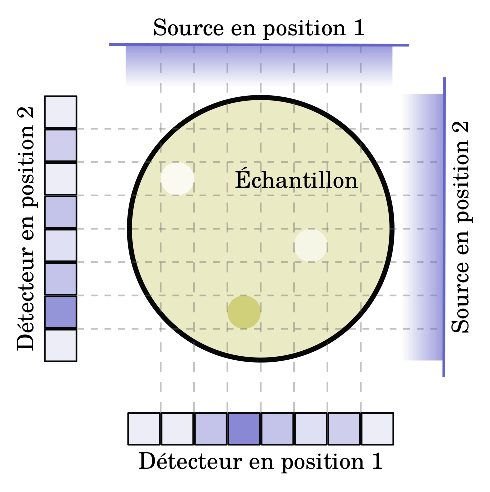
\includegraphics[]{principe_tomo.eps}
				\caption{\label{fig03:principe_tomo}Mise en évidence de la méthode de tomographie sur une coupe transversale d'un échantillon cylindrique : l'échantillon (ou l'appareillage) tourne sur l'axe normal au plan de la coupe de manière à prendre plusieurs radiographies.}
			\end{figure}
			\begin{figure}\centering
				\subfloat[]{
					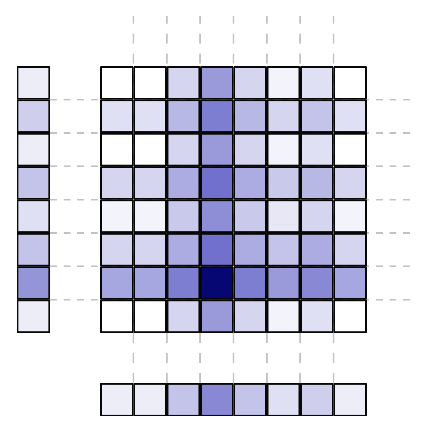
\includegraphics[]{reconstruction_tomo_00.eps}}\hspace{1cm}
				\subfloat[]{
					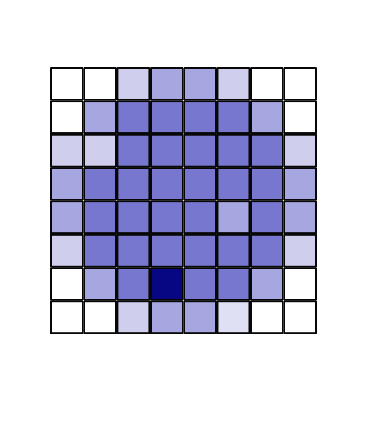
\includegraphics[]{reconstruction_tomo_01.eps}}
				\caption{\label{fig03:reconstruction_tomo}Méthode de reconstruction des images par superposition des radiographies : (a) résultat obtenu avec 2 positions différentes (cas de la figure \ref{fig03:principe_tomo}) et (b) avec un nombre bien plus grand de projections.}
			\end{figure}
			\\La reconstruction en tomographie, obtenue par superposition des projections, donne un champ scalaire tri-dimensionnel correspondant au champ d'absorption des rayons X dans l'espace. Tout comme un champ scalaire à deux dimensions peut être perçu comme une image dont chaque pixel correspond à un scalaire, le fichier de sortie de la tomographie peut se mettre sous la forme d'une image en trois dimensions où chaque voxel correspond à un scalaire. Il est alors possible de travailler sur ces images pour les améliorer et les analyser, c'est ce que nous allons voir dans le paragraphe suivant.
	\subsection{Traitements d'images 3D}\label{para03:traitement_image}
		Cette partie s'intéresse aux procédés numériques permettant de modifier les volumes donnés par la tomographie. Le lecteur peut se référer à \citet{bovik_handbook_2010} afin de mieux comprendre les processus de traitements d'images décrits dans la suite. Que ce soit en 2D ou en 3D, toute image est définie par un format déterminant la taille de l'image en fonction de ses dimensions. Nous ne considérerons que des images monochromatiques, donc ayant un seul canal (en niveaux de gris), de manière à ce que chaque pixel/voxel soit associé à un seul scalaire. L'élément unitaire constituant l'image sera dès à présent appelé voxel puisqu'une généralité pourra être faite aux images 3D. Le format s'exprime en "bit" et indique les valeurs qu'un voxel peut prendre. Par exemple, les voxels d'une image au format 8-bit ne peuvent prendre que $2^8$ soit $256$ valeurs : l'image sera constituée de voxels ayant des valeurs comprises entre 0 et 255 et dont la taille en mémoire vaut 1 octet. Une image 2D au format 16-bit (donc $2$ octets) de dimension $900\times 700$ aura des valeurs comprises entre $0$ et $2^{16}-1=65535$ et aura une taille en mémoire de $900\times 700\times 2=1260000$ octets. Les images issues de la tomographie et traitées dans cette thèse sont des images au format 8-bit en niveaux de gris. Elle pourraient être sauvegardées sous forme de matrices à trois dimensions directement lues par un langage de programmation ou un éditeur de texte mais cela ne s'avère pas pratique pour la visualisation. Généralement, les images 3D sont sauvegardées en couches, que l'on appelle aussi "stacks". En effet, les voxels étant orientés selon un repère orthonormal à trois dimensions, il est possible d'enregistrer les images en 2D (couche de 1 voxel) pour chaque couche normales à une direction du repère. Par exemple, une image de taille $M\times N\times H$ peut s'enregistrer sous forme de $H$ images de taille $M\times N$. Le visualisation se fait alors couche par couche de manière à pouvoir observer l'intégralité de l'échantillon.
		\\Un outil très utile en traitement et analyse d'images est l'histogramme. Il s'agit d'un type de graphe, souvent sous forme de barres verticales, qui indique pour chaque valeur d'intensité de voxel possible (en fonction du format de l'image) le nombre de voxels ayant cette valeur.
		\subsubsection{Binarisation par Seuillage}\label{para03:threshold}
			Les images en niveau de gris ont l'avantage de fournir plus ou moins d'information concernant le niveau d'absorption des rayons X au sein de l'échantillon. Cependant, pour de nombreuses tâches de post-traitement et d'analyse, cette information ne s'avère pas toujours utile. En effet, dans de nombreux cas il est utile de connaître uniquement les phases en présence. Ainsi, si l'échantillon est constitué de deux phases, ce que nous considérerons dans la suite, alors uniquement deux valeurs sont nécessaires pour définir l'image. Ces deux valeur peuvent par exemple être $0$ pour la phase constituant le vide (donc les pores) et $255$ pour la matière constituant les grains. Lorsque le matériau est biphasique il y a un autre avantage : on peut choisir de travailler sur des images binaires très légères au format "1-bit" prenant les valeurs $0$ ou $1$.
			\\Une méthode qui consiste à transformer une image quelconque en image binaire est une méthode de binarisation et se fait généralement par seuillage. Le seuillage consiste à déterminer une valeur seuil pour laquelle les voxels dont la valeur est inférieure prennent la première valeur binaire tandis que ceux dont la valeur est supérieure prennent l'autre valeur binaire. La détermination de cette valeur seuil peut se faire selon différentes méthodes, automatiques ou non.
			\\La méthode de binarisation la plus simple consiste à visualiser l'image binaire après chaque seuillage de manière à choisir, au choix de l'utilisateur, la valeur de seuil la plus cohérente avec le résultat attendu. Cette méthode est simple mais peut s'avérer également longue lorsque de nombreuses images sont à traiter. De plus, cette méthode est très dépendante de l'utilisateur. Afin de palier à ces problèmes, il existe plusieurs méthodes automatiques : ces dernières, bien qu'étant plus complexes d'un point de vue technique, sont très simples et très rapides à mettre en \oe{}uvre du point de vue de l'utilisateur et ne dépendent pas directement de l'utilisateur mais de l'allure de l'histogramme. Ces méthodes automatiques ont été employées et sont présentées au paragraphe \ref{para04:seuillage}.
		\subsubsection{Filtres binaires de bases}\label{para03:filtres}
			Toute personne ayant fait un minimum de traitement d'images a entendu parler de filtres. Un filtre est à l'image ce que l'opérateur algébrique est à la matrice - n'oublions pas qu'une image est une matrice. Cet opérateur numérique est capable de transformer l'image entièrement mais il est utilisé dans la très grande majorité des cas de manière itérative et sur des petites zones de l'image. Les zones de travail des filtres sont appelés noyaux ou éléments structurants et la taille de ces éléments ainsi que leur forme sont choisies par l'utilisateur. Chaque voxel de l'image se voit appliquer le filtre de la manière suivante : les voxels constituants le noyau par rapport au voxel en cours de traitement sont analysés afin de déterminer la nouvelle valeur de ce dernier. Le choix de la forme et de la taille de l'élément structurant aura un impact très fort sur le résultat, le nombre d'itération du filtre est également quelque chose d'important. Quelques filtres basiques, travaillant sur des images binaires (valeurs possibles : $0$ ou $1$, respectivement blanc et bleu sur la figure \ref{fig03:morpho_math}) vont être décrits ci-dessous :
			\begin{itemize}
				\item \'Erosion : s'il existe un voxel de l'élément structurant ayant la valeur $0$ (blanc) alors la valeur $0$ (blanc) est attribuée au voxel en cours d'analyse. Ce filtre donne plus d'importance aux voxels blancs proches des frontières entre les phases blanches et bleues. Si on considère les voxels $1$ (bleus) comme étant de la matière, alors ce filtre simule l'effet d'une érosion de la matière.
				\item Dilatation : il s'agit du filtre opposé à l'érosion. S'il existe dans le noyau un voxel de valeur $1$ (bleu) alors la valeur attribuée est $1$ (bleu). Cette fois-ci le filtre s'apparente à une dilatation de la matière.
				\item Ouverture : l'opération d'ouverture consiste à appliquer successivement une érosion puis une dilatation avec le même élément structurant. L'ouverture permet de supprimer les voxels bleus isolés dans les phases blanches.
				\item Fermeture : application successive d'une dilatation puis d'une érosion avec un même noyau. Il s'agit ici d'éliminer des petits groupes de voxels blancs isolés dans les phases bleues.
			\end{itemize}
			\begin{figure}\centering
				\subfloat[Image binaire d'origine]{
					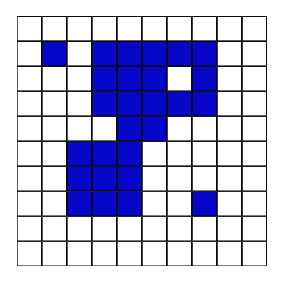
\includegraphics[scale=.8]{morpho_math_00.eps}}
				\subfloat[Noyau]{
					\hspace{1cm}
					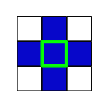
\includegraphics[scale=.8]{morpho_math_01.eps}
					\hspace{1cm}}\\
				\subfloat[\'Erosion]{
					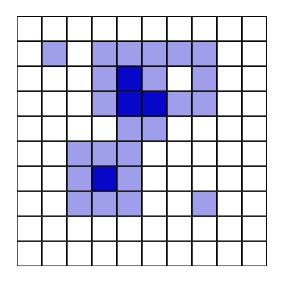
\includegraphics[scale=.8]{morpho_math_erosion.eps}}\hspace{3mm}
				\subfloat[Dilatation]{
					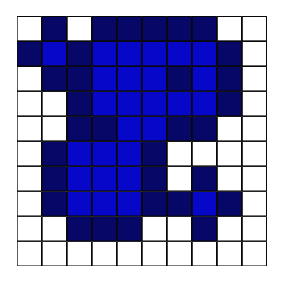
\includegraphics[scale=.8]{morpho_math_dilatation.eps}}\hspace{3mm}
				\subfloat[Ouverture]{
					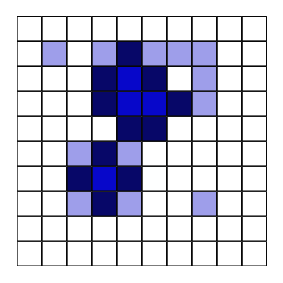
\includegraphics[scale=.8]{morpho_math_ouverture.eps}}\hspace{3mm}
				\subfloat[Fermeture]{
					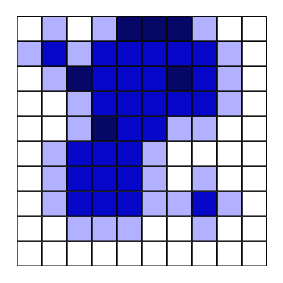
\includegraphics[scale=.8]{morpho_math_fermeture.eps}}
				\caption{\label{fig03:morpho_math}Effets des filtres morphologiques de base (c-f) sur une image binaire (a) en utilisant l'élément structurant (b). Les pixels en transparence sont ceux qui s'annulent (deviennent blancs), ceux qui apparaissent plus foncés sont ceux qui s'activent (deviennent bleus).}
			\end{figure}
			Les explications concernant ces filtres peuvent être trouvées dans les lectures de \citeauthor{heijmans_algebraic_1990} \citep{heijmans_algebraic_1990, ronse_algebraic_1991}. Ces filtres ne sont pas destinés uniquement aux images binaires puisqu'ils fonctionnent également sur des images en niveaux de gris. Une illustration des effets du filtre est présentée sur la figure \ref{fig03:morpho_math}.

		\subsubsection{Segmentation}
			La segmentation est le processus de reconnaissance du signal pour attribuer une identité, un label, à chaque partie du signal. C'est par un processus de segmentation qu'un code informatique est capable de reconnaître la morphologie ou l'intensité d'une certaine entité dans une image. Il existe de nombreuses méthodes de segmentation qui considèrent l'image comme une carte topologique et simulent des phénomènes naturels pour engendrer des structures géodésiques. De nombreux ouvrages destinés à la morphologie mathématique expliquent ces méthodes (\citet{haralick_image_1987} et \citet{dougherty_mathematical_1992} en sont des exemples).
			\\L'algorithme utilisé dans cette thèse est régulièrement utilisé pour la segmentation. Il s'agit de la méthode du "watershed" qui est illustrée sur la figure \ref{fig03:watershed}. Avec cette méthode, l'intensité des voxels peut être comparée à une altitude, les zones d'identification des grains à des lacs et la propagation de ces zones à une montée des eaux. Lorsque plusieurs lacs sont présents sur un profil altimétrique et qu'une montée des eaux se réalise, les lacs augmentent en taille en même temps qu'ils gagnent de l'altitude. Lorsque deux lacs se rejoignent au niveau d'un sommet alors une ligne de partage des eaux apparaît : c'est à cet endroit qu'une digue sera construite si le mélange des eaux n'est pas souhaité. Lorsque l'eau arrive sur un sommet mais que l'autre côté du sommet n'est pas immergé alors l'eau se propagera automatiquement de l'autre côté du sommet. Ce phénomène continue jusqu'à ce que la montée des eaux se termine.
			La méthode de segmentation par watershed fonctionne de manière identique. Dans une zone d'appartenance certaine à un grain, un marqueur est créé afin d'identifier ce grain (un lac est créé). Ce processus est réalisé pour chacun des grains dans la limite du possible. Chaque marqueur est unique : il en existe un seul par grain. Maintenant que chaque grain est identifié et existe, il est nécessaire de propager les marqueurs dans l'image afin qu'ils prennent la forme de chacun des grains (montée des eaux). La propagation est réalisée en fonction du champ d'intensité des voxels (profil altimétrique) : les voxels qui touchent les marqueurs et qui ont une intensité inférieure ou égale à celle du marqueur prennent la valeur du marqueur (inondation), ceux qui ont une intensité directement supérieure ne seront immergés que dans l'étape suivante. Lorsque deux marqueurs se rejoignent, ils restent indépendants et le processus peut continuer (création d'une digue). Le processus continue jusqu'à ce que les marqueurs atteignent une intensité définie comme valeur seuil d'appartenance aux grains.
			\begin{figure}\centering
				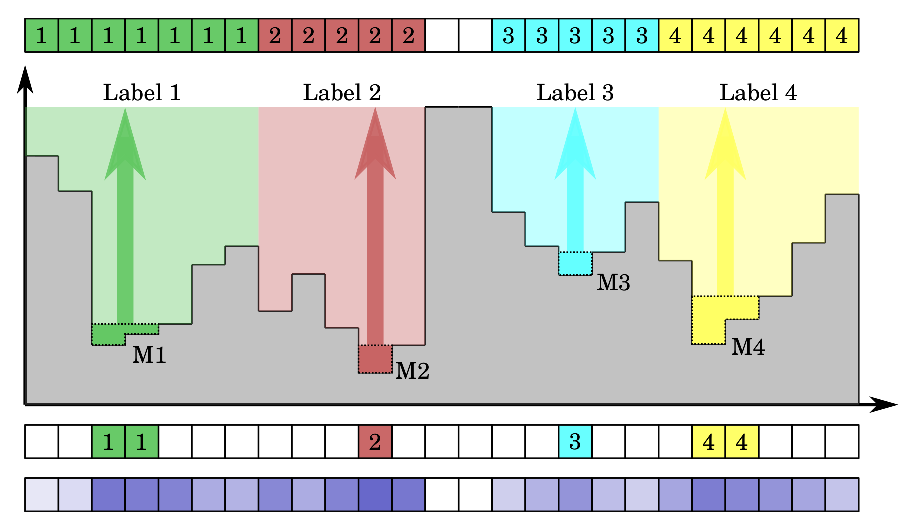
\includegraphics[]{watershed.eps}
				\caption{\label{fig03:watershed}Principe de segmentation par watershed (de bas en haut): signal sur une dimension ; masque des marqueurs (de même dimension que l'image) ; analogie géodésique : le signal donne l'altitude et les marqueurs sont des lacs, puis montée des eaux ; signal segmenté.}
			\end{figure}
	\subsection{Corrélation d'images numériques 3D}\label{para03:DIC}
		La corrélation d'images numériques (DIC pour Digital Image Correlation) est un outil puissant pour les mécaniciens puisqu'il permet de mesurer un champ cinématique hétérogène lors d'essais expérimentaux. Lors des essais, des photographies de l'échantillon sont prises au cours du temps de manière à observer les déplacements en surface d'échantillon en comparant les photographies. On voit de suite l'intérêt de la tomographie dans ce domaine : il est alors possible d'observer les déplacements dans un volume plutôt que dans un plan. On parle alors de corrélation de volumes numériques (DVC pour Digital Volume Correlation).
		\\Le principe de la corrélation d'images, qu'elles soient 2D ou 3D, se base sur la comparaison de deux images. Pour cela il est nécessaire de définir le coefficient de corrélation normalisé CCN qui est calculé pour comparer deux images $I_1$ et $I_2$:
		\begin{equation}\label{eq03:NCC}
			\mathrm{CCN} = \cfrac{\sum_{x,y,z} \left(I_1(x,y,z)\cdot I_2(x+u, y+v, z+w)\right)}{\sqrt{\sum_{x,y,z} I_1(x,y,z)\cdot \sum_{x,y,z} I_2(x+u, y+v, z+w)}}
		\end{equation}
		où $I_1(x,y,z)$ est la valeur en niveaux de gris du voxel de l'image de référence situé aux coordonnées $x$, $y$ et $z$ et $I_2$ est l'image à comparer, déplacée de $u$ suivant $x$, $v$ suivant $y$ et $w$ suivant $z$. Plus la valeur de ce coefficient à une valeur proche de $1$, plus la similarité entre les deux images est grande. Si $I_1$ et $I_2$ partagent exactement le même signal alors le coefficient de corrélation normalisé vaudra $1$.
		\\La mesure des champs de déplacements est basée sur la corrélation d'images. En effet, si on divise l'image d'origine en plusieurs images, plus petites, appelées "imagettes" et que l'on définit des zones de recherche des mêmes imagettes dans l'image à comparer alors il existe pour chaque zone de recherche un triplet $(u,v,w)$ qui maximise le coefficient de corrélation normalisé. Si ce coefficient maximal est proche de $1$ alors il est supposé que le déplacement subit par l'imagette est de $u$ voxels dans la direction $(Ox)$, $v$ voxels dans la direction $(Oy)$ et $w$ voxels dans la direction $(Oz)$. La connaissance de la taille des voxels indique la mesure réelle.
		\\Il est à noter que :
		\begin{itemize}
			\item Une image non contrastée et uniforme ne permettra pas de trouver un maximum pour CCN dans la zone de recherche puisque les signaux $I_1$ et $I_2$ seront quasi-identiques partout. Il faut des hétérogénéités, qu'elles soient naturelles ou artificielles.
			\item Plus les imagettes sont petites, meilleure est la résolution du champ de déplacement.
			\item La taille des imagettes dépend de la taille des hétérogénéités dans l'échantillon.
			\item Pour obtenir plus de précision concernant la mesure des déplacements, il est nécessaire de faire une interpolation 3D sur le volume. De base, la précision de la mesure est de l'ordre de la taille du voxel. Si on augmente le nombre de voxels alors la précision est également augmentée (au prix d'un calcul plus lourd).
			\item La corrélation ne peut se faire qu'entre deux imagettes quasi-identiques. Si la déformation de l'imagette entre l'image de référence et l'image à comparer est trop grande alors la corrélation sera mauvaise et le déplacement inconnu. Pour visualiser les déplacements sur des échantillons grandement déformés il est nécessaire de mesurer et sommer les déplacements sur des états successifs relativement proches (\textit{i.e.} pour des états dont la déformation n'évolue que faiblement).
		\end{itemize}
		Il existe d'autres types de mesures de corrélation mais celle présentée ici est sans nul doute la plus utilisée. De la même manière, il existe plusieurs méthodes algorithmiques permettant de mesurer les champs de déplacements. Le choix a été fait de se concentrer sur la méthode utilisée dans les travaux de cette thèse. Il est d'ailleurs utile de préciser que le code Tomowarp2 a été utilisé afin de mener les calculs de corrélation sur les images de tomographie. Une description de ce code est donnée par \citet{tudisco_tomowarp2_2017}.

\section{Simulations numériques des milieux granulaires}\label{para:methodes_simu}
	Les outils numériques permettent aux mécaniciens actuels de réduire significativement les campagnes d'essais grâce aux simulations numériques. Il est par exemple possible de mener dans le même temps plusieurs essais dont seuls quelques paramètres changent afin d'en étudier leur effet. Afin de s'assurer de la pertinence des résultats issus des simulations numériques, il est primordial que l'utilisateur du programme connaisse la méthode de simulation utilisée. En effet, il est nécessaire de savoir de quelle manière est discrétisée la géométrie de l'échantillon numérique, de quelle manière peuvent être attribuées les conditions aux limites, de quelle manière la loi de comportement des éléments a été créée ou encore de quelle manière les itérations de calculs sont définies.
	\\Globalement, les méthodes de simulation sont basées sur la discrétisation de la géométrie. Ainsi, un matériau réel qui est défini de manière continue sera approximé par un matériau dont les propriétés sont définies sur un certain nombre d'éléments. Nous allons, dans cette partie, nous concentrer sur des méthodes très utilisées en simulations mécaniques : les éléments discrets et les éléments finis.
	\subsection{Méthode des éléments discrets (DEM)}
		\subsubsection{Description de la méthode}
			La méthode des éléments discrets (DEM pour Discrete Element Method/Model) est une méthode qui a commencé à être réellement développée dans les années 1980 \citep{cundall_discrete_1979} mais qui s'est grandement popularisée à partir du milieu des années 1990. Il s'agit d'une méthode adaptée à la modélisation des milieux granulaires puisque les éléments discrets sont les particules constituant le milieu granulaire. Il y a donc autant d'éléments géométriques dans la simulation que de grains dans l'échantillon simulé. La DEM s'est construite essentiellement à partir de simulations faites sur les structures moléculaires. Les structures moléculaires étant constituées d'atomes, il est possible de les modéliser par un ensemble de sphères ayant un certain arrangement. Cet arrangement dépend de l'environnement puisque des forces interatomiques existent. La dynamique des sphères est donc très dépendante de cet environnement et il est possible de simuler le comportement d'un tel milieu grâce à ce qu'on appelle la dynamique moléculaire. Il existe cependant des différences considérables entre le modèle moléculaire et un milieu granulaire. En effet, les particules macroscopiques sont soumises à de la friction solide et engendre des interactions entre particules différentes des interactions entre atomes, qui eux, subissent des forces normales dérivant de potentiels.
			\\On distingue différentes méthodes parmi les méthodes DEM \citep{cambou_micromechanics_2009}, entre autre :
			\begin{itemize}
				\item les méthodes \emph{smooth DEM} pour lesquelles les interactions intergranulaires sont décrites par des fonctions continues et suffisamment différentiables. Les méthodes de dynamique moléculaire décrites plus haut font parties de la smooth DEM. \citet{cundall_discrete_1979} a également exposé des travaux réalisés avec cette méthode en utilisant des systèmes de ressorts et d'amortisseurs pour décrire les forces d'interaction de contact.
				\item les méthodes \emph{non smooth DEM} pour lesquelles les interactions intergranulaires sont décrites par des lois de choc ou toute autre relation décrivant les sauts de vitesse et les seuils de force. L'approche la plus utilisée est sans doute celle des contacts dynamiques développée par \citet{moreau_unilateral_1988} et \citet{jean_unilaterality_1992}.
			\end{itemize}
			La liste qui précède n'est pas une liste exhaustive des méthodes de simulation par DEM. Le lecteur pourra aisément s'informer sur d'autres méthodes \citep{bardet_introduction_1998}, mais également mieux connaître les différences entre les méthodes "smooth" et "non smooth" en se rapportant à la lecture de \citet{wolf_modelling_1996}.
			\\La figure \ref{fig03:principe_DEM} illustre le principe de la simulation par éléments discrets.
			\begin{figure}\centering
				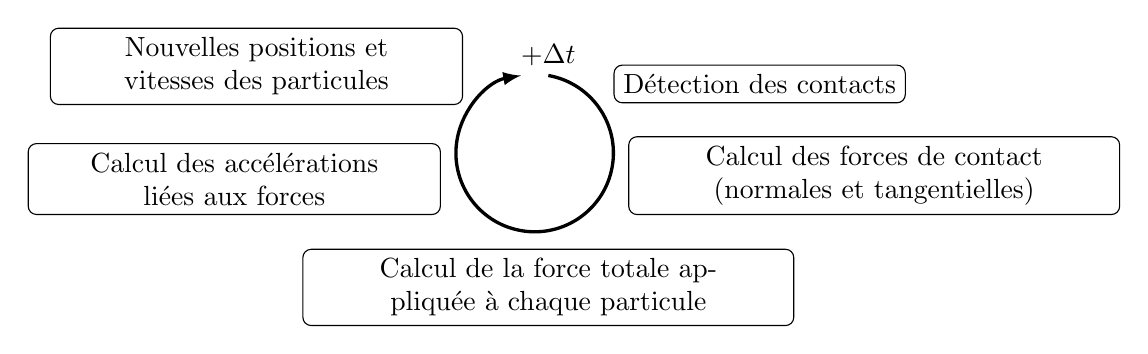
\begin{tikzpicture}
					\tikzset{court/.style={draw, rectangle, rounded corners=3pt},
							 long/.style={draw, rectangle, rounded corners=3pt, text centered}}
					\draw[->, >=latex, very thick] (0,1) arc (80:-260:1);
					\node[above] (increment) at (0,1) {$+\Delta t$};
					\node[court, above right] (contacts) at (38:1.05) {Détection des contacts};
					\node[long, right, text width=6cm] (forces) at (-15:1.05) {Calcul des forces de contact (normales et tangentielles)};
					\node[long, below, text width=6cm] (total) at (-90:1.2) {Calcul de la force totale appliquée à chaque particule};
					\node[long, left, text width=5cm] (accelerations) at (-167:1.4) {Calcul des accélérations liées aux forces};
					\node[long, above left, text width=5cm] (nouveau) at (150:1.25) {Nouvelles positions et vitesses des particules};
				\end{tikzpicture}
				\caption{\label{fig03:principe_DEM}Méthode de simulation par éléments discrets}
			\end{figure}
		\subsubsection{Matériaux et géométries employés}
			Le principal objectif de la méthode des éléments discrets et de pouvoir simuler un milieu granulaire suffisamment volumineux pour connaître la réponse mécanique du milieu à l'échelle macroscopique. En ayant connaissance du nombre de particules nécessaires pour décrire le comportement d'un milieu granulaire, on s'aperçoit vite des limitations liées aux outils numériques. Il faut pouvoir modéliser un très grand nombre de particules, ayant chacune plusieurs degrés de liberté et plusieurs contacts. Pour cette raison, la très grande majorité des simulations sont réalisées sur des collections de grains de formes relativement simples et régulières (disques, sphères, polyèdres réguliers) afin de modéliser les grains par un minimum de points représentatifs.
			\\De par la nature indéformable des éléments discrets, la méthode DEM est largement utilisée dans les problèmes d'écoulements granulaires, pour lesquels la déformation physique des grains est négligeable \citep{vu-quoc_accurate_1999, vu-quoc_normal_2001, wu_experimental_2003}. Cependant, en utilisant un loi de contact adaptée, la méthode montre également son utilité dans l'étude de la densification des matériaux granulaires comme le montre les travaux de \citet{heyliger_cold_2001, martin_study_2003, martin_study_2003-1, skrinjar_discrete_2004} au début des années 2000.
		\subsubsection{Limites de la méthode}
			Les simulations par DEM ont leurs avantages mais présentent également une limite majeure pour l'étude des grains déformables. En effet, une fois fixée au départ de la simulation, la géométrie des grains reste la même durant la simulation. Malgré les méthodes mises en place pour modéliser la déformation des grains en DEM, le changement de forme des particules n'est pas pris en compte. De cette manière, pour un matériau granulaire dont les grains sont déformables, et pour de grandes déformations des grains, la réponse mécanique réelle du milieu peut être assez différente de la simulation.
	\subsection{Méthode des éléments finis (FEM)}
		\subsubsection{Description de la méthode}
			La méthode des éléments finis (FEM pour Finite Element Method) est une méthode couramment utilisée en calcul des structures pour la conception et le dimensionnement. La méthode n'est pas uniquement dédiée aux structures puisqu'elle est capable de résoudre un large éventail de problèmes : structurels, thermiques, électromagnétiques, fluidiques, en linéaire, en non linéaire, en stationnaire ou en transitoire. On voit ici la puissance de la méthode et on comprend l'intérêt des ingénieurs et chercheurs dans l'utilisation d'outils utilisant cette méthode. La méthode a commencé à se développer dans les années 1940 avec les travaux de \citet{hrennikoff_solution_1941} et \citet{courant_variational_1943}. Le principe de base de la méthode FEM consiste à discrétiser un milieu continu en un ensemble d'éléments de géométrie connue et dont les propriétés sont définies en amont de la simulation. La génération d'un maillage adapté est nécessaire pour modéliser au mieux une structure continue en un nombre fini d'éléments. Chaque point singulier d'un élément fini est appelé n\oe{}ud. Ce sont les n\oe{}uds qui possèdent un certain nombre de degrés de liberté et permettent à la structure de se mouvoir sous l'action de forces. Une des méthode de résolution couramment utilisée est celle de Rayleigh-Ritz et consiste à minimiser l'énergie potentielle du système en la décrivant comme la différence entre l'énergie de déformation et le travail des forces volumiques et/ou surfaciques. Cette minimisation de l'énergie donne généralement une équation de la forme :
			\begin{equation}\label{eq03:equation_FEM}
				[K]\cdot \{Q\} - \{F\} = 0 \qquad \Leftrightarrow \qquad [K]\cdot \{Q\} = \{F\}
			\end{equation}
			où $[K]$ est la matrice raideur, $\{Q\}$ est le vecteur donnant les différents degrés de liberté et $\{F\}$ est le vecteur des forces appliquées aux n\oe{}uds. Avec cette équation, pour chaque n\oe{}ud, il est possible de connaître la force appliquée (ou résultante) et le déplacement imposé (ou résultant). On obtient ainsi des champs de force et de déplacement plus ou moins proches des champs réels en faisant une interpolation sur chaque élément fini.
			\\La méthode de simulation par éléments finis est décrite sur la figure \ref{fig03:methode_FEM}. Une première étape consiste à calculer la matrices de raideur et le vecteur de charges pour chaque élément du maillage dans les repères locaux. Ensuite, une nouvelle boucle est faite sur les éléments du maillage afin de déterminer la matrice de passage entre le repère local et le repère global ; à partir de cette matrice de passage, la matrice de raideur et le vecteur de charge sont exprimées dans le repère global. Une matrice d'assemblage est ensuite créée de manière à reconstruire les matrices et vecteurs du système dans son intégralité (avec tous les degrés de liberté). L'équation (\ref{eq03:equation_FEM}) peut finalement être résolue de manière à connaître les forces et déplacements en tout n\oe{}ud de la structure maillée et les efforts internes peuvent être calculés. Si le lecteur s'intéresse plus particulièrement à la méthode FEM, il peut se reporter à la lecture de \citet{cazenave_methode_2013}.
			\begin{figure}\centering
				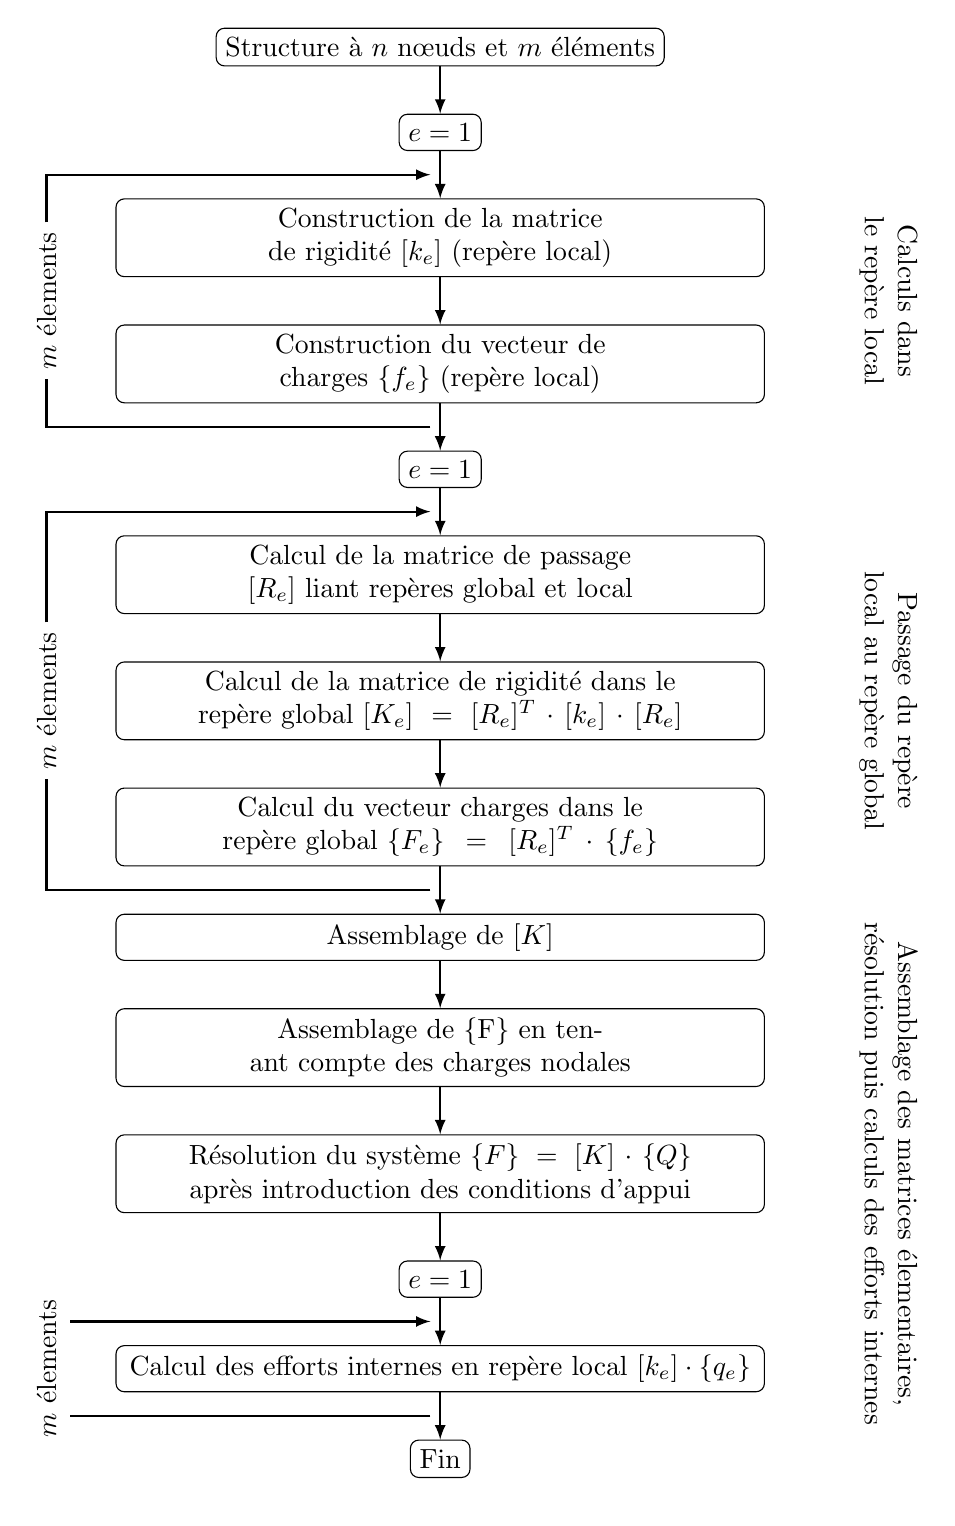
\begin{tikzpicture}
					\tikzset{etape/.style={draw, rectangle, below, rounded corners=3pt, text centered}}
					\tikzset{long/.style={draw, rectangle, below, rounded corners=3pt, text width=8cm, text centered}}
					\tikzset{fleche/.style={->, >=latex, thick}}
					\tikzset{increment/.style={rotate=90}}
					\tikzset{explication/.style={above, text width=4cm, text centered, rotate=-90, shift={(0,5.2)}}}
					\node[etape] (Structure)at(0,0){Structure à $n$ n\oe{}uds et $m$ éléments};
					\node[etape, shift={(0,-.6)}] (Init1)at(Structure.south){$e=1$};
					\node[long, shift={(0,-.6)}] (local1)at(Init1.south){Construction de la matrice de rigidité $[k_e]$ (repère local)};
					\node[long, shift={(0,-0.6)}] (local2)at(local1.south){Construction du vecteur de charges $\{f_e\}$ (repère local)};
					\node[etape, shift={(0,-0.6)}] (Init2)at(local2.south){$e=1$};
					\node[long, shift={(0,-0.6)}] (global1)at(Init2.south){Calcul de la matrice de passage $[R_e]$ liant repères global et local};
					\node[long, shift={(0,-0.6)}] (global2)at(global1.south){Calcul de la matrice de rigidité dans le repère global $[K_e]=[R_e]^T\cdot [k_e]\cdot [R_e]$};
					\node[long, shift={(0,-0.6)}] (global3)at(global2.south){Calcul du vecteur charges dans le repère global $\{F_e\}=[R_e]^T\cdot \{f_e\}$};
					\node[long, shift={(0,-0.6)}] (assemblage1)at(global3.south){Assemblage de $[K]$};
					\node[long, shift={(0,-0.6)}] (assemblage2)at(assemblage1.south){Assemblage de \{F\} en tenant compte des charges nodales};
					\node[long, shift={(0,-0.6)}] (resolution)at(assemblage2.south){Résolution du système $\{F\}=[K]\cdot \{Q\}$ après introduction des conditions d'appui};
					\node[etape, shift={(0,-0.6)}] (Init3)at(resolution.south){$e=1$};
					\node[long, shift={(0,-0.6)}] (interne)at(Init3.south){Calcul des efforts internes en repère local $[k_e]\cdot\{q_e\}$};
					\node[etape, shift={(0,-0.6)}] (fin)at(interne.south){Fin};
					\node[increment, shift={(-.3,5)}] (iter1)at(local1.south){$m$ élements};
					\node[increment, shift={(0,5)}] (iter2)at(global2.center){$m$ élements};
					\node[increment, shift={(0,5)}] (iter3)at(interne.center){$m$ élements};
					\node[shift={(0,-.3)}] (iter1haut)at(Init1.south){}; \node[shift={(0,-.3)}] (iter1bas)at(local2.south){};
					\node[shift={(0,-.3)}] (iter2haut)at(Init2.south){}; \node[shift={(0,-.3)}] (iter2bas)at(global3.south){};
					\node[shift={(0,-.3)}] (iter3haut)at(Init3.south){}; \node[shift={(0,-.3)}] (iter3bas)at(interne.south){};
					\draw[fleche] (Structure) -- (Init1); \draw[fleche] (Init1) -- (local1); \draw[fleche] (local1) -- (local2);
					\draw[fleche] (local2) -- (Init2); \draw[fleche] (Init2) -- (global1); \draw[fleche] (global1) -- (global2);
					\draw[fleche] (global2) -- (global3); \draw[fleche] (global3) -- (assemblage1);
					\draw[fleche] (assemblage1) -- (assemblage2); \draw[fleche] (assemblage2) -- (resolution);
					\draw[fleche] (resolution) -- (Init3); \draw[fleche] (Init3) -- (interne); \draw[fleche] (interne) -- (fin);
					\draw[fleche] (iter1bas) -| (iter1) |- (iter1haut);
					\draw[fleche] (iter2bas) -| (iter2) |- (iter2haut);
					\draw[thick] (iter3bas) -- ++(-4.7,0); \draw[<-, >=latex, thick] (iter3haut) -- ++(-4.7,0);
					\node[explication] (expl2) at (global2.center) {Passage du repère local au repère global};
					\node[explication, shift={(-.3,0)}] (expl1) at (local2.north) {Calculs dans le repère local};
					\node[above, text width=8cm, text centered, rotate=-90, shift={(0,5.2)}] (expl3) at (resolution.center) {Assemblage des matrices élementaires, résolution puis calculs des efforts internes};
				\end{tikzpicture}
				\caption{\label{fig03:methode_FEM}Organigramme générale de résolution par la méthode FEM (cas d'un calcul en statique) \citep{cazenave_methode_2013}}
			\end{figure}
		\subsubsection{Matériaux et géométries employés}
			La méthode des éléments finis est une méthode de simulation utilisée pour les structures continues. En effet, le principe de la méthode FEM est d'approximer au mieux le comportement d'un milieu continu en le discrétisant. Les champs en sortie de simulation sont interpolés de manière à obtenir des champs continus. La génération d'un maillage approprié est indispensable pour rendre la méthode efficace. Plus les éléments du maillage seront petits, plus longs seront les temps de calculs mais meilleure sera la solution puisque l'approximation se rapproche alors du modèle continu. En plus de la densité du maillage, le choix des éléments constituant le maillage est important. C'est en effet en fonction de leur géométrie et de leurs propriétés qu'il est possible de simuler certains comportements avec une plus ou moins grande précision.
			\\Les progrès réalisé en informatique ces dernière décennies (puissance de calculs et interactions homme/machine notamment) ont permis d'évoluer vers des méthodes sophistiquées qui ne s'arrêtent plus aux cas de la statique linéaire. De nombreux bureaux d'études travaillent aujourd’hui sur des problèmes de statique non linéaire et même de dynamique non linéaire.
		\subsubsection{Limites de la méthode}
			De très nombreux calculs sont nécessaires pour résoudre un problème de calcul de structure par éléments finis. En fonction de la méthode utilisée, à chaque élément du maillage est associé un certain nombre de vecteurs et matrices qui doivent être calculés et assemblés dans des vecteurs ou matrices bien plus grands dont la taille dépend du nombre de degrés de liberté du problème. Cela se passe à chaque incrément de temps pour des calculs en dynamique ou quasi-statique. Pour cette raison, les simulations de structures complexes - nécessitant donc un maillage fin - subissant de larges déformations vont demander une très grande puissance de calcul et de stockage informatique. Il est donc important de savoir optimiser la méthode à partir d'hypothèses fondées (définition d'un incrément de temps, choix de la densité du maillage, etc.).
			\\Une étape indispensable à la méthode des éléments finis est celle de la génération du maillage qui n'est pas toujours évidente et pose souvent des problèmes aux ingénieurs en bureaux d'études. En effet, il est primordial de savoir choisir le type d'élément définissant le maillage en fonction des simulations et de savoir gérer, dans le même temps, la densité du maillage. Certaines parties de la géométrie des structures modélisées peuvent nécessiter un maillage très fin alors que la plus grande partie de cette structure peut être définie par un maillage assez grossier. Dans ce cas, le travail technique consiste à faire un maillage qui prend en compte de nombreux facteurs. Ces facteurs peuvent être plus ou moins bien connus et pondérés par un logiciel informatique mais c'est souvent l'expérience et les connaissances du technicien sur le modèle qui vont permettre de générer un maillage approprié. La méthode FEM est donc très dépendante de l'utilisateur.
	\subsection{Méthode des éléments finis multi-particules (MP-FEM)}
		\label{para03:MPFEM}
		\subsubsection{Description de la méthode}
			La méthode des éléments finis multi-particules (MP-FEM pour Multi-Particules Finite Element Method) est basée sur la méthode FEM mais s'intéresse également aux interactions existantes entre différentes particules de la même manière qu'avec la méthode DEM. Les travaux de \citet{ransing_powder_2000}, \citeauthor{gethin_numerical_2001} \citep{gethin_numerical_2001, gethin_two_2006} et \citet{lewis_combined_2005} réalisés au début des années 2000 font partie des premiers travaux utilisant cette méthode sur des matériaux granulaires déformables. Toutefois, les simulations concernées par ces premiers travaux étaient en 2D. Depuis, la méthode MP-FEM n'a cessé de se développer grâce aux travaux de \citet{procopio_simulation_2005} et aux premières simulations 3D apparues en 2007 avec les travaux de \citet{chen_numerical_2007} et \citeauthor{frenning_efficient_2008} \citep{frenning_efficient_2008, frenning_compression_2010}. Peu d'années après, \citet{schmidt_simulation_2010} et \citet{harthong_study_2012} utilisent les éléments finis pour étudier la plasticité des grains par l'obtention des surfaces de charge. \citet{gustafsson_multi_2013} va même jusqu'à reproduire les phénomènes de fissuration lors de la compression de particules de minerai de fer. Plus récemment, la méthode a été utilisée par \citeauthor{guner_numerical_2015} \citep{guner_numerical_2015, guner_effects_2018} afin d'étudier la compaction d'une poudre de cuivre et de mieux comprendre les effets des paramètres de compression (vitesse de chargement, lubrification, température). \citet{loidolt_modeling_2018} a, quant à lui, utilisée la méthode MP-FEM dans le but d'observer l'effet des forces de contact cohésives entre les grains sur la surface de charge. \citet{feng_cohesive_2019} couple la MP-FEM avec la méthode de zone cohésive afin de simuler les fissuration dans des grains d'aluminium et de chlorure de sodium.
			\\Le principe de la méthode repose sur les principes des éléments discrets et des éléments finis. La figure \ref{fig03:DEM_MPFEM} illustre la manière dont est discrétisé un milieu granulaire avec la méthode MP-FEM (schéma de droite) comparée à celle de la méthode DEM (schéma de gauche). La discrétisation de la matière se fait par l'intermédiaire d'éléments finis. Ainsi, chaque particule est définie de la même manière qu'une structure dans un modèle éléments finis. La différence avec la méthode FEM intervient lorsqu'un assemblage de particules et d'interactions entre elles est créé de la même manière qu'avec la méthode DEM. En effet, des lois de contact sont définies entre les différents matériaux et sont appliquées lorsqu'un contact entre particules a été détecté.
			\\La méthode MP-FEM permet d'analyser la compression d'un empilement de grains sous des conditions de chargement quasi-statiques. L'expérience montre que l'utilisation d'un schéma d'intégration explicite dans le code commercial utilisé permet une convergence des simulations numériques d'empilements avec de nombreux contacts et de grandes déformations des particules. Ce schéma d'intégration n'exclut aucunement les erreurs de calcul et, pour cette raison, une comparaison des résultats numériques et expérimentaux est nécessaire. Cette méthode a l'avantage de prendre en compte l'évolution de la géométrie des particules au cours de la simulation et de fournir de nombreuses informations à l'intérieur des particules (champs de contraintes et de déformations notamment).
			\\Afin de valider la méthode MP-FEM, \citeauthor{chen_contribution_2008} \cite{chen_contribution_2008} a mené une campagne d'essais expérimentaux et numériques sur la compression de particules de plomb. La méthode de validation est basée sur la comparaison des résultats numériques et expérimentaux. Pour cela, l'auteur a comprimé un certain nombre de particules (seules ou dans un ensemble de particules) dans une presse hydraulique puis a mené des simulations numériques, avec la méthode MP-FEM, sur des géométries similaires à celles de l'expérimentation, avec des conditions de chargement identiques et une loi de comportement associée au matériau plomb. La comparaison des résultats expérimentaux et numériques montre l'efficacité de la méthode dans la simulation de la compression d'un empilement de particules très déformables. Cette efficacité a même été démontrée jusqu'à l'obtention d'un milieu dont la densité relative atteint \num{0.92} (la densité relative initiale étant proche de \num{0.60}).
			\begin{figure}\centering
				\includegraphics[width=0.8\textwidth]{DEM_MPFEM.png}
				\caption{\label{fig03:DEM_MPFEM}Illustration 2D des méthodes DEM (à gauche) et MP-FEM (à droite). Les éléments discrets sont indéformables et l'étude des contacts en surface des éléments, avec une loi de contact adaptée, est utilisée. Les éléments finis sont déformables, les champs de déformations et contraintes sont connus au sein des grains et les contacts en surface sont pris en compte avec une loi de contact adaptée. Illustration issue des travaux de thèse de \citet{harthong_modelisation_2010}.}
			\end{figure}
		\subsubsection{Matériaux et géométries employés}
			Par définition, tout comme la méthode des éléments discrets, la méthode MP-FEM est adaptée aux milieux granulaires. Le fait de générer un maillage pour chaque particule permet d'utiliser une bibliothèque de grains très diversifiée. Il est ainsi possible de modéliser le milieu granulaire avec des grains dont la géométrie est assez complexe et évolue au cours de temps.
		\subsubsection{Limites de la méthode}
			Bien que la possibilité de simuler un matériau granulaire avec des grains dont la géométrie est complexe soit un avantage de la méthode des éléments finis multi-particules, cette méthode hérite également des limites de la méthode des éléments finis. En effet, en fonction de la complexité des grains, un nombre plus ou moins important de n\oe{}uds va être nécessaire et, en fonction de la puissance de calcul disponible, le nombre de grains dans le milieu granulaire modélisé s'en retrouve limité. Pour une même puissance de calcul, une collection de grains pour la méthode MP-FEM sera généralement plus petite qu'une collection de grains pour la méthode des éléments discrets. En revanche, avec les éléments finis multi-particules, la déformation des grains est prise en compte dans le processus de simulation.
		
		\paragraph{}
		Il a été vu les nombreux avantages d'utiliser la méthode des éléments finis multi-particules dans le cadre de la simulation numérique de la compression des milieux granulaires dont les grains sont de nature déformable. Les moyens numériques ne cessent d'évoluer pour permettre des puissances de calculs toujours plus importantes et l'utilisation de mémoire toujours plus grande. Pour ces raisons, la méthode MP-FEM est vouée à être de plus en plus utilisée dans l'analyse de la compression des milieux granulaires. Cependant, les résultats actuels sur l'utilisation de cette méthode sont encore relativement pauvres comparé aux méthodes FEM et DEM. C'est la raison pour laquelle une méthode est développée dans cette thèse pour utiliser les éléments finis multi-particules sur une microstructure réelle afin de l'intégrer dans un code éléments finis et générer des simulations numériques pouvant être comparées directement aux essais expérimentaux.
		\\Quelques travaux basés sur une approche similaire ont été réalisés. En effet, l'utilisation de la tomographie pour intégrer une structure réelle dans une simulation par éléments finis a par exemple été observé dans les travaux de \citet{youssef_finite_2005} sur des matériaux cellulaires et \citet{wautier_linking_2015} sur la neige. \Citet{vlahinic2013} ont, quant à eux, menés des simulations DEM à partir d'informations obtenues par imagerie 3D. Cependant, au moment de la rédaction de ce manuscrit, l'auteur n'a pas connaissance de travaux pour lesquels les éléments finis multi-particules sont utilisés pour simuler le comportement mécanique d'un ensemble de particules déformables en interactions entre elles à partir des géométries réelles des particules et des conditions de chargement réellement observées par des méthodes d'imagerie 3D.